\documentclass[review]{elsarticle}
\usepackage{lineno}
\usepackage{hyperref}
\usepackage{graphicx}
\usepackage{todonotes}
\usepackage{amsthm}

\modulolinenumbers[5]

\journal{International Journal of Approximate Reasoning}

% correct bad hyphenation here
\hyphenation{op-tical net-works semi-conduc-tor}

\newtheorem{theorem}{Theorem}

\theoremstyle{definition}
\newtheorem{definition}{Definition}

%%%%%%%%%%%%%%%%%%%%%%%
%% Elsevier bibliography styles
%%%%%%%%%%%%%%%%%%%%%%%
%% To change the style, put a % in front of the second line of the current style and
%% remove the % from the second line of the style you would like to use.
%%%%%%%%%%%%%%%%%%%%%%%

%% Numbered
%\bibliographystyle{model1-num-names}

%% Numbered without titles
%\bibliographystyle{model1a-num-names}

%% Harvard
%\bibliographystyle{model2-names.bst}\biboptions{authoryear}

%% Vancouver numbered
%\usepackage{numcompress}\bibliographystyle{model3-num-names}

%% Vancouver name/year
%\usepackage{numcompress}\bibliographystyle{model4-names}\biboptions{authoryear}

%% APA style
%\bibliographystyle{model5-names}\biboptions{authoryear}

%% AMA style
%\usepackage{numcompress}\bibliographystyle{model6-num-names}

%% `Elsevier LaTeX' style
\bibliographystyle{elsarticle-num}
%%%%%%%%%%%%%%%%%%%%%%%

\begin{document}

\begin{frontmatter}

\title{Possibilistic Testing of OWL Axioms\\ Against RDF Data%\tnoteref{mytitlenote}
}
%\tnotetext[mytitlenote]{My title note.}

\author[I3S]{Andrea G. B. Tettamanzi}
\ead{andrea.tettamanzi@unice.fr}

\author[I3S]{Catherine Faron-Zucker}
\ead{faron@unice.fr}

\author[I3S]{Fabien Gandon}
\ead{fabien.gandon@inria.fr}

\address[I3S]{Universit\'e C\^ote d'Azur, Inria, CNRS, I3S, 2000, route des Lucioles, Sophia Antipolis, France}

\begin{abstract}
We develop the theory of a possibilistic framework for OWL~2 axiom testing against RDF datasets,
as an alternative to statistics-based heuristics. The intuition behind it is to evaluate the credibility of OWL~2 axioms based on the \emph{evidence} available
in the form of a set of facts contained in a chosen RDF dataset. To achieve it, we first define the notions of development, content, support, confirmation and counterexample of an axiom. Then we use these notions to define the possibility and necessity of an axiom and its acceptance/rejection index combining both of them. 
Finally, we report a practical application of the proposed framework to test \texttt{SubClassOf} axioms against the DBpedia RDF dataset.
\end{abstract}

\begin{keyword}
Possibility Theory \sep Linked Data \sep Ontology Learning \sep OWL~2 \sep Axioms
\end{keyword}

\end{frontmatter}

\linenumbers

\section{Introduction}

Ontology learning~\cite{MaedcheStaab2001} is a broad field of research, aiming at
overcoming the knowledge acquisition bottleneck through
the automatic generation of ontologies, that has started to emerge at the beginning
of this century, mainly within the context of the semantic Web.
The input for ontology learning can be text in natural language or
existing ontologies (typically expressed in OWL) and instance data (typically
represented in RDF)~\cite{LehmannVoelker2014}.
In the former case, the focus is on the population of ontologies with facts
derived from text using natural language processing methods, although
the generation of lightweight taxonomies can also be undertaken.
In the latter case, which is the one we are interested in,
induction-based methods like the ones developed in
inductive logic programming and data mining are developed to detect meaningful
patterns and learn schema axioms from existing instance data (facts) and
their metadata, if available.

On a related note, there exists a need for evaluating and validating ontologies,
be they the result of an analysis effort or of a semi-automatic learning method,
and/or validating instance data.
Indeed, instead of starting from the \emph{a priori} assumption that a given ontology
is correct and verify whether the facts contained in an RDF base satisfy it,
one may treat ontologies like hypotheses and develop a methodology to verify
whether the RDF facts corroborate or falsify them. Ontology learning and validation
are thus strictly related.
They could even be seen as an agile and test-driven approach to ontology development,
where the linked data is used as a giant test case library not only to validate the
schema but even to suggest new developments.

Both ontology learning and ontology/data validation rely critically on (candidate) axiom scoring. To see why, let us consider the following example.
While constructing an ontology for a given domain (say, politics),
based on the description of instances in a given dataset, e.g., DBpedia,
we might suspect that a mayor is an elected representative. Before we insert this
knowledge into the ontology, we should score the corresponding axiom
\texttt{SubClassOf(Mayor ElectedRepresentative)} against the statements in the
dataset, i.e., measure the extent to which it is compatible with them.
Conversely, for validation, imagine that an ontology about politics models the fact that plurality of offices
is banned, through a set of axioms like \texttt{SubClassOf(Mayor ObjectComplementOf(MP))}. In order to check whether a given country obeys this rule, we might score
the above axiom against the linked open government data of that country.

In this paper, we will tackle the problem of testing a single, isolated axiom,
which is anyway the first step to solve the problem of validating an entire ontology.

This article is organized as follows:
Section~\ref{related-work} discusses related work on ontology learning and validation. Section~\ref{principles} presents the principles of axiom testing and
Section~\ref{critique-of-probabilistic-scoring} discusses the difficulties and
shortcomings of conventional probability-based scoring heuristics, which motivate
the search for an alternative.
Section~\ref{possibility-theory}
presents our proposal of an axiom scoring heuristics based on possibility theory.
A computational framework for axiom scoring based on such heuristics is then
presented in Section~\ref{OWL2SPARQL} and evaluated on \texttt{SubClassOf} axioms.
Section~\ref{conclusion} draws some conclusions and gives directions for future work.

\section{Related Work}\label{related-work}

Recent contributions towards the automatic creation of OWL~2 ontologies
from large repositories of RDF facts include
FOIL-like algorithms for learning concept definitions~\cite{FanizziDAmatoEsposito2008},
statistical schema induction via association rule mining~\cite{FleischhackerVoelkerStuckenschmidt2012},
and light-weight schema enrichment methods based on the DL-Learner
framework~\cite{HellmannLehmannAuer2009,BuehmannLehmann2012}.
All these methods apply and extend techniques developed within inductive logic programming
(ILP)~\cite{ILPat20}. For a recent survey of the wider field of ontology learning,
see~\cite{LehmannVoelker2014}.

The growing need for evaluating and validating ontologies is witnessed by general methodological investigations~\cite{GangemiCatenacciCiaramitaLehmann2005,GangemiCatenacciCiaramitaLehmann2006}, 
surveys~\cite{TartirBudakArpinarSheth2007} and tools like OOPS!~\cite{PovedaSuarezGomez2012}
for detecting pitfalls in ontologies.
Ontology engineering methodologies, such as METHONTOLOGY~\cite{FernandezGomezJuristo1997},
distinguish two validation activities, namely verification (through formal methods, syntax, logics, etc.)
and validation through usage. Whilst this latter is usually thought of as user studies,
an automatic process of validation based on RDF data would provide a cheap and scalable assistance,
whereby the existing linked data may be regarded as usage traces that can be used
to test and improve the ontologies, much like log mining can be used to provide
test cases for development in the replay approaches.
Alternatively, one may regard the ontology as a set of integrity constraints and check if the
data satisfy them, using a tool like Pellet integrity constraint validator (ICV),
which translates OWL ontologies into SPARQL queries to automatically validate RDF data~\cite{SirinTao2009}. 
The RDF Data Shapes W3C Working Group has been created in 2014 and published in 2017 a working draft, intended to become a W3C recommendation, of the SHACL Shapes Constraint Language, a language for validating RDF graphs against a set of structural conditions.\footnote{https://www.w3.org/TR/shacl/}
A similar approach also underlies the idea of test-driven evaluation of linked data 
quality~\cite{KontokostasWestphalAuerHellmannLehmannCornelissen2014}.
To this end, OWL ontologies are interpreted under the closed-world assumption and
the weak unique name assumption. 

%Fabien
%ICV was among the proposals to create the RDF Data Shapes Working Group. Interestingling a result of your work could also be to generate candidate Shapes.

The most popular scoring heuristics proposed in the literature are based
on statistical inference (see, e.g., \cite{BuehmannLehmann2012}).
As such a probability-based framework is not always completely satisfactory,
we have recently proposed~\cite{TettamanziFaronZuckerGandon2014ekaw,%
TettamanziFaronZuckerGandon2015kcap}
an axiom scoring heuristics based on a formalization in possibility theory of
the notions of logical content of a theory and of falsification, loosely inspired
by Karl Popper's approach to epistemology, and working with an open-world semantics.
In this article, we justify such proposal and we develop a theory of OWL axiom
testing against RDF facts based on possibility theory, whose output is
a degree of possibility and necessity of an axiom, given the available evidence.
Our proposal is coherent with a recently proposed possibilistic extension of
description logics~\cite{QiPanJi2011,QiJiPanDu2010}.

In particular, our first attempts~\cite{TettamanziFaronZuckerGandon2014ekaw}
pointed out that a possibilistic approach to test candidate axioms
could be beneficial to ontology learning, as well as to ontology and
knowledge base validation, although at the cost of a heavier computational
cost than the probabilistic scores it aims to complement.
Further investigation~\cite{TettamanziFaronZuckerGandon2015kcap} showed that
time capping can alleviate the computation of the proposed possibilistic
axiom scoring heuristics without giving up the precision of the scores.

\section{Principles of OWL 2 Axiom Testing}\label{principles}

The problem we study may be stated as follows:
given a \emph{hypothesis} about the relations holding among some entities of a domain,
syntactically expressed in the form of an OWL~2 axiom,
we wish to evaluate its credibility based on the \emph{evidence} available
in the form of a set of facts contained in an RDF dataset and, therefore,
syntactically expressed in RDF. We call this task \emph{axiom testing}.

If, for a moment, we abstract away from the particular syntax of the hypothesis
and of the available evidence, what we have here is a fundamental problem in
epistemology, with important ramifications in statistical inference,
data mining, inductive reasoning, medical diagnosis,
judicial decision making, and even the philosophy of science.
Central to this problem is the notion of \emph{confirmation}:
see \cite{Crupi2016} for a general overview of the major approaches to
confirmation theory in contemporary philosophy.
All the approaches build on logical entailment (from evidence to the hypothesis
or from the hypothesis to evidence, to which background knowledge may be added).
The approach we follow may be classified as a form of extended
hypothetico-deductivism, whereby, roughly speaking, evidence $e$ confirms
a hypothesis $h$ if the latter entails it, $h \models e$, and disconfirms it
if the former entails the negation of the latter, $e \models \neg h$.
As we will see, other considerations will be added to extend this basic idea.

Testing an OWL 2 axiom against an RDF dataset can thus be done by checking
whether the formulas entailed by it are confirmed by the facts
contained in the RDF dataset.\footnote{Note that calling linked data search engines
like Sindice could virtually extend the dataset to the whole LOD cloud.}
The rest of this section will be devoted to formalizing and developing
this intuition.

\subsection{OWL 2 Direct Model-Theoretic Semantics and Development of OWL 2 Axioms}
We refer to the model-theoretic semantics of OWL~2 as defined in~\cite{OWL2-direct-semantics}.\footnote{http://www.w3.org/TR/2012/REC-owl2-direct-semantics-20121211/, \\Section 2.2 Interpretations}
An interpretation $\mathcal{I}$ for a datatype map $D$ and a vocabulary $V$ over $D$ is defined by an interpretation domain $\Delta^\mathcal{I}=\Delta_{I}\cup\Delta_{D}$  ($\Delta_{I}$ is the \textit{object domain} and $\Delta_{D}$ the \textit{data domain}), and a valuation function $\cdot^{\mathcal{I}}$ with seven restrictions: $\cdot^{C}$ mapping class expressions to subsets of $\Delta_{I}$,  $\cdot^{OP}$ mapping object properties to subsets of $\Delta_{I}\times\Delta_{I}$, $\cdot^{DP}$ mapping data properties to subsets of $\Delta_{I}\times\Delta_{D}$, $\cdot^{I}$ mapping individuals to elements of $\Delta_{I}$, $\cdot^{DT}$ mapping datatypes to subsets of $\Delta_{D}$, $\cdot^{LT}$ mapping literals to elements of $\Delta_{D}$ and $\cdot^{FT}$ mapping facets to subsets of $\Delta_{D}$.

Table~\ref{tab:term-semantics} provides a reference of the model-theoretic semantics
of OWL~2 expressions.

\begin{table}
\caption{The model-theoretic semantics of OWL~2 expressions.
The first column gives the OWL~2 functional syntax of the expression,
the second column its more compact $\mathcal{SHOIQ}$ description logic syntax,
and the last column shows its semantics.\label{tab:term-semantics}}
\begin{center}\scriptsize
\begin{tabular}{|l|l|l|}
\hline
  OWL~2 Functional Syntax & DL Syntax & Interpretation \\
\hline &&\\[-0.95em]\hline
  $\mathsf{ObjectInverseOf}(R)$ & $R^-$ &
    $(R^-)^\mathcal{I} = \{\langle y, x \rangle \mid \langle x, y \rangle \in R^\mathcal{I} \}$ \\
\hline
  $\mathsf{DataIntersectionOf}(D_1\ \ldots\ D_n)$ & $D_1 \sqcap \ldots \sqcap D_n$  &
    $D_1^\mathcal{I} \cap \ldots \cap D_n^\mathcal{I}$ \\
  $\mathsf{DataUnionOf}(D_1\ \ldots\ D_n)$ & $D_1 \sqcup \ldots \sqcup D_n$  &
    $D_1^\mathcal{I} \cup \ldots \cup D_n^\mathcal{I}$ \\
  $\mathsf{DataComplementOf}(D)$ & $\neg D$ & $\mathtt{D}^{\mathrm{arity}(D)} \setminus D^\mathcal{I}$ \\
  $\mathsf{DataOneOf}(d_1\ \ldots\ d_n)$ & $\{d_1, \ldots, d_n\}$ &
    $\{d_1^\mathcal{I}, \ldots, d_n^\mathcal{I}\}$ \\
  $\mathsf{DatatypeRestriction}(D\ F_1\ d_1\ \ldots\ F_n\ d_n)$ &  &
    $D^\mathcal{I} \cap \langle F_1, d_1\rangle^\mathcal{I} \cap \ldots \cap \langle F_n, d_n\rangle^\mathcal{I}$  \\
\hline
  $\mathsf{ObjectIntersectionOf}(C_1\ \ldots\ C_n)$ & $C_1 \sqcap \ldots \sqcap C_n$ &
    $C_1^\mathcal{I} \cap \ldots \cap C_n^\mathcal{I}$ \\
  $\mathsf{ObjectUnionOf}(C_1\ \ldots\ C_n)$ & $C_1 \sqcup \ldots \sqcup C_n$ &
    $C_1^\mathcal{I} \cup \ldots \cup C_n^\mathcal{I}$ \\
  $\mathsf{ObjectComplementOf}(C)$ & $\neg C$ & $\Delta^\mathcal{I} \setminus C^\mathcal{I}$ \\
  $\mathsf{ObjectOneOf}(a_1\ \ldots\ a_n)$ & $\{a_1, \ldots, a_n\}$ & $\{a_1^\mathcal{I}, \ldots, a_n^\mathcal{I}\}$ \\
  $\mathsf{ObjectSomeValuesFrom}(R\ C)$ & $\exists R.C$  &
    $\{x \mid \exists y.\langle x, y\rangle \in R^\mathcal{I} \land y \in C^\mathcal{I}\}$ \\
  $\mathsf{ObjectAllValuesFrom}(R\ C)$ & $\forall R.C$ &
    $\{x \mid \forall y.\langle x, y\rangle \in R^\mathcal{I} \Rightarrow y \in C^\mathcal{I}\}$ \\
  $\mathsf{ObjectHasValue}(R\ a)$ & $\exists R.\{a\}$ &
    $\{x \mid \langle x, a^\mathcal{I}\rangle \in R^\mathcal{I}\}$ \\
  $\mathsf{ObjectHasSelf}(R)$ & $\exists R.\mathsf{Self}$ &
    $\{x \mid \langle x, x\rangle \in R^\mathcal{I}\}$ \\
  $\mathsf{ObjectMinCardinality}(n\ R)$ & $\geq nR.\top$ &
    $\{x \mid \|\{y \mid \langle x, y\rangle \in R^\mathcal{I}\}\| \geq n\}$ \\
  $\mathsf{ObjectMaxCardinality}(n\ R)$ & $\leq nR.\top$ &
    $\{x \mid \|\{y \mid \langle x, y\rangle \in R^\mathcal{I}\}\| \leq n\}$ \\
  $\mathsf{ObjectExactCardinality}(n\ R)$ & $=nR.\top$ &
    $\{x \mid \|\{y \mid \langle x, y\rangle \in R^\mathcal{I}\}\| = n\}$ \\
  $\mathsf{ObjectMinCardinality}(n\ R\ C)$ & $\geq nR.C$ &
    $\{x \mid \|\{y \mid \langle x, y\rangle \in R^\mathcal{I} \land y \in C^\mathcal{I}\}\| \geq n\}$ \\
  $\mathsf{ObjectMaxCardinality}(n\ R\ C)$ & $\leq nR.C$ &
    $\{x \mid \|\{y \mid \langle x, y\rangle \in R^\mathcal{I} \land y \in C^\mathcal{I}\}\| \leq n\}$ \\
  $\mathsf{ObjectExactCardinality}(n\ R\ C)$ & $=nR.C$ &
    $\{x \mid \|\{y \mid \langle x, y\rangle \in R^\mathcal{I} \land y \in C^\mathcal{I}\}\| = n\}$ \\
\hline
  $\mathsf{DataSomeValuesFrom}(R\ D)$ & $\exists R.D$  &
    $\{x \mid \exists y.\langle x, y\rangle \in R^\mathcal{I} \land y \in D^\mathcal{I}\}$ \\
  $\mathsf{DataAllValuesFrom}(R\ D)$ & $\forall R.D$ &
    $\{x \mid \forall y.\langle x, y\rangle \in R^\mathcal{I} \Rightarrow y \in D^\mathcal{I}\}$ \\
  $\mathsf{DataHasValue}(R\ d)$ & $\exists R.d$ &
    $\{x \mid \langle x, d^\mathcal{I}\rangle \in R^\mathcal{I}\}$ \\
  $\mathsf{DataMinCardinality}(n\ R)$ & $\geq nR.\top$ &
    $\{x \mid \|\{y \mid \langle x, y\rangle \in R^\mathcal{I}\}\| \geq n\}$ \\
  $\mathsf{DataMaxCardinality}(n\ R)$ & $\leq nR.\top$ &
    $\{x \mid \|\{y \mid \langle x, y\rangle \in R^\mathcal{I}\}\| \leq n\}$ \\
  $\mathsf{DataExactCardinality}(n\ R)$ & $=nR.\top$ &
    $\{x \mid \|\{y \mid \langle x, y\rangle \in R^\mathcal{I}\}\| = n\}$ \\
  $\mathsf{DataMinCardinality}(n\ R\ D)$ & $\geq nR.D$ &
    $\{x \mid \|\{y \mid \langle x, y\rangle \in R^\mathcal{I} \land y \in D^\mathcal{I}\}\| \geq n\}$ \\
  $\mathsf{DataMaxCardinality}(n\ R\ D)$ & $\leq nR.D$ &
    $\{x \mid \|\{y \mid \langle x, y\rangle \in R^\mathcal{I} \land y \in D^\mathcal{I}\}\| \leq n\}$ \\
  $\mathsf{DataExactCardinality}(n\ R\ D)$ & $=nR.D$ &
    $\{x \mid \|\{y \mid \langle x, y\rangle \in R^\mathcal{I} \land y \in D^\mathcal{I}\}\| = n\}$ \\
\hline
\end{tabular}
\end{center}
\end{table}

Table~\ref{tab:axiom-semantics} provides a reference of the semantics
of the 32 axiom types of OWL~2.

\begin{table}
\caption{The model-theoretic semantics of OWL~2 axioms. The first column gives the OWL~2 Functional syntax of the
axiom, the second column its more compact $\mathcal{SHOIQ}$ description logic syntax,
and the last column shows it semantics.%, for all $x$, $y$, and $z$.
\label{tab:axiom-semantics}}
\begin{center}\scriptsize
\begin{tabular}{|l|l|l|}
\hline
  OWL~2 Functional Syntax & DL Syntax & Semantics \\
\hline &&\\[-0.95em]\hline
  $\mathsf{SubClassOf}(C\ D)$ & $C \sqsubseteq D$  & $C^\mathcal{I} \subseteq D^\mathcal{I}$ \\
  $\mathsf{EquivalentClasses}(C_1\ \ldots\ C_n)$ & $C_i \equiv C_j$, $i,j \in \{1, \ldots n\}$ & 
    $C_i^\mathcal{I} = C_j^\mathcal{I}$, $i,j \in \{1, \ldots n\}$ \\
  $\mathsf{DisjointClasses}(C_1\ \ldots\ C_n)$ & $\mathsf{Dis}(C_1, \ldots, C_n)$ &
    $C_i^\mathcal{I} \cap C_j^\mathcal{I} = \emptyset$, $i,j \in \{1, \ldots n\}$, $i\neq j$  \\
  $\mathsf{DisjointUnion}(C\ C_1\ \ldots\ C_n)$ & $C \equiv C_1 \sqcup \ldots \sqcup C_n$, and &
    $C^\mathcal{I} = C_1^\mathcal{I} \cup \ldots \cup C_n^\mathcal{I}$, and \\
  & $\mathsf{Dis}(C_1, \ldots, C_n)$ &
    $C_i^\mathcal{I} \cap C_j^\mathcal{I} = \emptyset$, $i,j \in \{1, \ldots n\}$, $i\neq j$  \\
\hline
  $\mathsf{SubObjectPropertyOf}(S, R)$ & $S \sqsubseteq R$ & $S^\mathcal{I} \subseteq R^\mathcal{I}$ \\
  $\mathsf{SubObjectPropertyOf}(w, R)$, with & $S_1\ldots S_n \sqsubseteq R$ &
    $S_1^\mathcal{I} \circ \ldots \circ S_n^\mathcal{I} \subseteq R^\mathcal{I}$,
    i.e., $\forall y_0, \ldots, y_n$, \\
  \quad$w = \mathsf{ObjectPropertyChain}(S_1\ \ldots\ S_n)$ & &
    $\langle y_0, y_1\rangle \in S_1^\mathcal{I} \land \ldots \land
    \langle y_{n-1}, y_n\rangle \in S_n^\mathcal{I}$ \\
  & & $\Rightarrow \langle y_0, y_n\rangle \in R^\mathcal{I}$ \\
  $\mathsf{EquivalentObjectProperties}(R_1\ \ldots\ R_n)$ & $R_i \equiv R_j$, $i,j \in \{1, \ldots n\}$ & 
    $R_i^\mathcal{I} = R_j^\mathcal{I}$, $i,j \in \{1, \ldots n\}$ \\
  $\mathsf{DisjointObjectProperties}(R_1\ \ldots\ R_n)$ & $\mathsf{Dis}(R_1, \ldots, R_n)$ &
    $R_i^\mathcal{I} \cap R_j^\mathcal{I} = \emptyset$, $i,j \in \{1, \ldots n\}$, $i\neq j$ \\
  $\mathsf{ObjectPropertyDomain}(R\ C)$ & $\geq 1 R \sqsubseteq C$ &
    $\langle x, y\rangle \in R^\mathcal{I} \Rightarrow x\in C^\mathcal{I}$ \\
  $\mathsf{ObjectPropertyRange}(R\ C)$ & $\top \sqsubseteq \forall R.C$ & 
    $\langle x, y\rangle \in R^\mathcal{I} \Rightarrow y\in C^\mathcal{I}$ \\
  $\mathsf{InverseObjectProperties}(S\ R)$ & $S \equiv R^-$ &
    $S^\mathcal{I} = \{\langle y, x \rangle \mid \langle x, y \rangle \in R^\mathcal{I} \}$ \\
  $\mathsf{FunctionalObjectProperty}(R)$ & $\mathsf{Fun}(R)$ &
    $\langle x, y\rangle \in R^\mathcal{I} \land \langle x, z\rangle \in R^\mathcal{I}
    \Rightarrow y = z$ \\
  $\mathsf{InverseFunctionalObjectProperty}(R)$ & $\mathsf{Fun}(R^-)$ &
    $\langle x, y\rangle \in R^\mathcal{I} \land \langle z, y\rangle \in R^\mathcal{I}
    \Rightarrow x = z$ \\
  $\mathsf{ReflexiveObjectProperty}(R)$ & $\mathsf{Ref}(R)$ & $\langle x, x\rangle \in R^\mathcal{I}$ \\
  $\mathsf{IrreflexiveObjectProperty}(R)$ & $\mathsf{Irr}(R)$ & $\langle x, x\rangle \notin R^\mathcal{I}$ \\
  $\mathsf{SymmetricObjectProperty}(R)$ & $\mathsf{Sym}(R)$ &
    $\langle x, y\rangle \in R^\mathcal{I} \Rightarrow \langle y, x\rangle \in R^\mathcal{I}$ \\
  $\mathsf{AsymmetricObjectProperty}(R)$ & $\mathsf{Asy}(R)$ &
    $\langle x, y\rangle \in R^\mathcal{I} \Rightarrow \langle y, x\rangle \notin R^\mathcal{I}$ \\
  $\mathsf{TransitiveObjectProperty}(R)$ & $\mathsf{Tra}(R)$ & 
    $\langle x, y\rangle \in R^\mathcal{I} \land \langle y, z\rangle \in R^\mathcal{I} \Rightarrow
    \langle x, z\rangle \in R^\mathcal{I}$ \\
\hline
  $\mathsf{SubDataPropertyOf}(S, R)$ & $S \sqsubseteq R$ & $S^\mathcal{I} \subseteq R^\mathcal{I}$ \\
  $\mathsf{EquivalentDataProperties}(R_1\ \ldots\ R_n)$ & $R_i \equiv R_j$, $i,j \in \{1, \ldots n\}$ & 
    $R_i^\mathcal{I} = R_j^\mathcal{I}$, $i,j \in \{1, \ldots n\}$ \\
  $\mathsf{DisjointDataProperties}(R_1\ \ldots\ R_n)$ & $\mathsf{Dis}(R_1, \ldots, R_n)$ &
    $R_i^\mathcal{I} \cap R_j^\mathcal{I} = \emptyset$, $i,j \in \{1, \ldots n\}$, $i\neq j$ \\
  $\mathsf{DataPropertyDomain}(R\ C)$ & $\geq 1 R \sqsubseteq C$ &
    $\langle x, y\rangle \in R^\mathcal{I} \Rightarrow x\in C^\mathcal{I}$ \\
  $\mathsf{DataPropertyRange}(R\ D)$ & $\top \sqsubseteq \forall R.D$ & 
    $\langle x, y\rangle \in R^\mathcal{I} \Rightarrow y\in D^\mathcal{I}$ \\
  $\mathsf{FunctionalDataProperty}(R)$ & $\mathsf{Fun}(R)$ &
    $\langle x, y\rangle \in R^\mathcal{I} \land \langle x, z\rangle \in R^\mathcal{I}
    \Rightarrow y = z$ \\
\hline
  $\mathsf{DatatypeDefinition}(T\ D)$ & $T \equiv D$ & $T^\mathcal{I} = D^\mathcal{I}$ \\
\hline
  $\mathsf{HasKey}(C\ (R_1\ \ldots\ R_n)\ (S_1\ \ldots\ S_m))$ & $\mathsf{Key}(C) =$ &
    $a, b\in C^\mathcal{I}$\quad$a, a_i, b, b_i$ named individuals \\
  \quad with $R_i$ object properties & $\{R_1, \ldots, R_n, S_1, \ldots, S_m\}$ & $\land \langle a, a_i\rangle \in R_i^\mathcal{I}
       \land \langle b, b_i\rangle \in R_i^\mathcal{I}$ \\
  \quad and $S_i$ data properties & & $\land \langle a, d_i\rangle \in S_i^\mathcal{I}
       \land \langle b, e_i\rangle \in S_i^\mathcal{I} \Rightarrow a = b$ \\
\hline
  $\mathsf{SameIndividual}(a_1\ \ldots\ a_n)$ & $a_i \doteq a_j$, $i,j\in\{1, \ldots, n\}$ &
    $a_i^\mathcal{I} = a_j^\mathcal{I}$, $i,j \in \{1, \ldots n\}$ \\
  $\textsf{DifferentIndividuals}(a_1\ \ldots\ a_n)$ & $a_i \not\doteq a_j$, $i,j\in\{1, \ldots, n\}$, $i\neq j$ &
    $a_i^\mathcal{I} \neq a_j^\mathcal{I}$, $i,j \in \{1, \ldots n\}$, $i\neq j$ \\
  $\mathsf{ClassAssertion}(C\ a)$ & $C(a)$ & $a^\mathcal{I} \in C^\mathcal{I}$ \\
  $\mathsf{ObjectPropertyAssertion}(R\ a\ b)$ & $R(a, b)$ &
    $\langle a^\mathcal{I}, b^\mathcal{I}\rangle \in R^\mathcal{I}$ \\
  $\mathsf{NegativeObjectPropertyAssertion}(R\ a\ b)$ & $\neg R(a, b)$ &
    $\langle a^\mathcal{I}, b^\mathcal{I}\rangle \notin R^\mathcal{I}$ \\
  $\mathsf{DataPropertyAssertion}(R\ a\ d)$ & $R(a, d)$ &
    $\langle a^\mathcal{I}, d^\mathcal{I}\rangle \in R^\mathcal{I}$ \\
  $\mathsf{NegativeDataPropertyAssertion}(R\ a\ d)$ & $\neg R(a, d)$  &
    $\langle a^\mathcal{I}, d^\mathcal{I}\rangle \notin R^\mathcal{I}$ \\
\hline
\end{tabular}
\end{center}
\end{table}

We aim at operationalizing the model-theoretic semantics of OWL~2 axioms into corresponding first-order logic formulas which will serve as a basis to query an RDF dataset in order to test OWL~2 candidate axioms against it. 
It was proposed by Hempel~\cite{Hempel1943}
that, given some body of evidence,
a hypothesis $\phi$ can be developed into a finite ground formula, which he
calls the \emph{development} of the hypothesis.
It is useful to recall Hempel's proposal first, which we will then adapt
to RDF + OWL~2.

Let $\mathcal{L}$ be a finite first-order language;
let $e, h\in\mathcal{L}$ be the available evidence and a hypothesis, respectively; let $C$ be a finite set of individual constants of $\mathcal{L}$
(typically, those occurring non-vacuously in $e$).
The \emph{development} of hypothesis $h$ according to $C$ is the formula $D_C(h)$,
such that $h \models D_C(h)$,
defined recursively as follows: Let $\phi, \psi\in\mathcal{L}$,
\begin{enumerate}
\item if $C = \emptyset$ or $\phi$ is atomic, then $D_C(\phi) = \phi$;
\item otherwise,
  \begin{enumerate}
  \item $D_C(\neg\phi) = \neg D_C(\phi)$;
  \item $D_C(\phi \lor \psi) = D_C(\phi) \lor D_C(\psi)$;
  \item $D_C(\phi \land \psi) = D_C(\phi) \land D_C(\psi)$;
  \item $D_C(\forall x\phi) = \bigwedge_{c\in C}D_C(\phi\{c/x\})$;
  \item $D_C(\exists x\phi) = \bigvee_{c\in C}D_C(\phi\{c/x\})$.
  \end{enumerate}
\end{enumerate}
In the above definition, $\phi\{c/x\}$ stands for the formula obtained
from $\phi$ by substituting all free occurrences of variable $x$ with constant $c$.

We can observe that $D_C(\phi)$, as defined above, can always be transformed
either into conjunctive normal form (CNF) or disjunctive normal form (DNF) by repeated
application of the De Morgan Laws, i.e.
\begin{equation}
  D_C(\phi) = \bigwedge_i \psi_i
  \quad\mbox{or}\quad
  D_C(\phi) = \bigvee_i \psi_i.
\end{equation}
In either case, the ground formulas $\psi_i$, which we may call
\emph{basic statements}, may be tested directly against the available facts
to compute a degree of corroboration of hypothesis $\phi$.

We shall now define the notion of \emph{development} of an OWL~2 axiom
with respect to an RDF dataset. That notion relies on a transformation,
which translates an OWL~2 axiom into a first-order logic formula based on the
set-theoretic formulas of the OWL direct semantics.%
\footnote{This transformation is similar to the two mappings defined in~\cite{DLHandbook2003}
(pages 154--155) to show the equivalence of DL and a two-variable fragment
of first-order logic.}

\begin{definition}\label{def:FOL-transform}
  Let $t(\cdot; x, y)$ be recursively defined as follows, with an OWL~2
  entity, expression, or axiom as the first argument
  and $x$, $y$ variables:
  \begin{itemize}
  \item Entities:
    \begin{itemize}
    \item if $d$ is a data value (a literal), $t(d; x, y) = (x = d)$;
    \item if $a$ is an individual name (an IRI), $t(a; x, y) = (x = a)$;
    \item if $C$ is an atomic concept, $t(C; x, y) = C(x)$;
    \item if $D$ is an atomic datatype, $t(D; x, y) = D(x)$;
    \item if $R$ is an atomic relation, $t(R; x, y) = R(x, y)$;
    \end{itemize}
  \item Expressions:
    \begin{itemize}
    \item $t(R^-; x, y) = t(R; y, x)$;
    \item $t(D_1 \sqcap \ldots \sqcap D_n; x, y) = t(D_1; x, y) \land \ldots \land t(D_n; x, y)$;
    \item $t(D_1 \sqcup \ldots \sqcup D_n; x, y) = t(D_1; x, y) \lor \ldots \lor t(D_n; x, y)$;
    \item $t(\neg D; x, y) = \neg t(D; x, y)$;
    \item $t(\{d_1, \ldots, d_n\}; x, y) = t(d_1; x, y) \lor \ldots \lor t(d_n; x, y)$;
    \item $t(C_1 \sqcap \ldots \sqcap C_n; x, y) = t(C_1; x, y) \land \ldots \land t(C_n; x, y)$;
  \item $t(C_1 \sqcup \ldots \sqcup C_n; x, y) = t(C_1; x, y) \lor \ldots \lor t(C_n; x, y)$;
  \item $t(\neg C; x, y) = \neg t(C; x, y)$;
  \item $t(\{a_1, \ldots, a_n\}; x, y) = t(a_1; x, y) \lor \ldots \lor t(a_n; x, y)$;
  \item $t(\exists R.C; x, y) = \exists y(t(R; x, y) \land t(C; y, z))$;
  \item $t(\forall R.C; x, y) = \forall y(\neg t(R; x, y) \lor t(C; y, z))$;
  \item $t(\exists R.\{a\}; x, y) = t(R; x, a)$;
  \item $t(\exists R.\mathsf{Self}; x, y) = t(R; x, x)$;
  \item $t(\geq nR.\top; x, y) = (\|\{y \mid t(R; x, y) \}\| \geq n)$;
  \item $t(\leq nR.\top; x, y) = (\|\{y \mid t(R; x, y) \}\| \leq n)$;
  \item $t(=nR.\top; x, y) = (\|\{y \mid t(R; x, y) \}\| = n)$;
  \item $t(\geq nR.C; x, y) = (\|\{y \mid t(R; x, y) \land t(C; y, z) \}\| \geq n)$;
  \item $t(\leq nR.C; x, y) = (\|\{y \mid t(R; x, y) \land t(C; y, z) \}\| \leq n)$;
  \item $t(=nR.C; x, y) = (\|\{y \mid t(R; x, y) \land t(C; y, z) \}\| = n)$;
  \item $t(\exists R.D; x, y) = \exists y(t(R; x, y) \land t(D; y, z))$;
  \item $t(\forall R.D; x, y) = \forall y(\neg t(R; x, y) \lor t(D; y, z))$;
  \item $t(\exists R.\{d\}; x, y) = t(R; x, d)$;
  \item $t(\geq nR.D; x, y) = (\|\{y \mid t(R; x, y) \land t(D; y, z) \}\| \geq n)$;
  \item $t(\leq nR.D; x, y) = (\|\{y \mid t(R; x, y) \land t(D; y, z) \}\| \leq n)$;
    \item $t(=nR.D; x, y) = (\|\{y \mid t(R; x, y) \land t(D; y, z) \}\| = n)$;
    \end{itemize}
  \item Axioms:
    \begin{itemize}
    \item $t(C_1 \sqsubseteq C_2; x, y) = \forall x(\neg t(C_1; x, y) \lor t(C_2; x, y))$; 
  \item $t(C_1 \equiv C_2; x, y) = \forall x((t(C_1; x, y) \land t(C_2; x, y)) \lor
    (\neg t(C_1; x, y) \land \neg t(C_2; x, y)))$;
  \item $t(\mathsf{Dis}(C_1, \ldots, C_n); x, y) =
    \bigwedge_{i = 1}^n\bigwedge_{j = i + 1}^n(\neg t(C_i; x, y) \lor \neg t(C_j; x, y))$;
  \item $t(C \equiv C_1 \sqcup \ldots \sqcup C_n, \mathsf{Dis}(C_1, \ldots, C_n); x, y) = t(C \equiv C_1 \sqcup \ldots \sqcup C_n; x, y) \land t(\mathsf{Dis}(C_1, \ldots, C_n); x, y)$;
  \item $t(S \sqsubseteq R; x, y) = \forall x\forall y(\neg t(S; x, y) \lor t(R; x, y))$;
  \item $t(S_1\ldots S_n \sqsubseteq R; x, y) =
    \forall x\forall z_1\ldots\forall z_{n - 1}\forall y
    (\neg t(S_1; x, z_1) \lor \neg t(S_2; z_1, z_2) \lor \ldots \lor \neg t(S_n; z_{n - 1}, y) \lor t(R; x, y))$;
  \item $t(R_1 \equiv R_2; x, y) = \forall x\forall y
    ((t(R_1; x, y) \land t(R_2; x, y)) \lor (\neg t(R_1; x, y) \land \neg t(R_2; x, y)))$;
  \item $t(\mathsf{Dis}(R_1, \ldots, R_n); x, y) =
    \bigwedge_{i = 1}^n\bigwedge_{j = i + 1}^n(\neg t(R_i; x, y) \lor \neg t(R_j; x, y))$;
  \item $t(\geq 1 R \sqsubseteq C; x, y) = \forall x\forall y
    (\neg t(R; x, y) \lor t(C; x, y))$;
  \item $t(\top \sqsubseteq \forall R.C) = \forall x\forall y
    (\neg t(R; x, y) \lor t(C; y, z))$;
  \item $t(S \equiv R^-; x, y) = \forall x\forall y
    ((t(S; x, y) \land t(R; y, x)) \lor (\neg t(S; x, y) \land \neg t(R; y, x)))$;
  \item $t(\mathsf{Fun}(R); x, y) = \forall x\forall y\forall z
    (\neg t(R; x, y) \lor \neg t(R; x, z) \lor y = z)$;
  \item $t(\mathsf{Fun}(R^-); x, y) = \forall x\forall y\forall z
    (\neg t(R; x, y) \lor \neg t(R; z, y) \lor x = z)$;
  \item $t(\mathsf{Ref}(R); x, y) = \forall x (t(R; x, x))$;
  \item $t(\mathsf{Irr}(R); x, y) = \forall x (\neg t(R; x, x))$;
  \item $t(\mathsf{Sym}(R); x, y) = \forall x\forall y
    (\neg t(R; x, y) \lor t(R; y, x))$;
  \item $t(\mathsf{Asy}(R); x, y) = \forall x\forall y
    (\neg t(R; x, y) \lor \neg t(R; y, x))$;
  \item $t(\mathsf{Tra}(R); x, y) = \forall x\forall y\forall z
    (\neg t(R; x, y) \lor \neg t(R; y, z) \lor t(R; x, z))$;
  \item $t(\top \sqsubseteq \forall R.D) = \forall x\forall y
    (\neg t(R; x, y) \lor t(D; y, z))$;
  \item $t(T \equiv D; x, y) = \forall x((t(T; x, y) \land t(D; x, y)) \lor
    (\neg t(T; x, y) \land \neg t(D; x, y)))$;
  \item $t(\mathsf{Key}(C) = \{R_1, \ldots, R_n\}; x, y) =
    \forall x\forall z\forall z_1\ldots\forall az_n
    (\neg t(C; x, y) \lor t(C; z, y) \lor
      \bigvee_{i = 1}^n(\neg R_i(x, z_i) \lor \neg R_i(z, z_i))
    \lor x = z)$;
  \item $t(a \doteq b; x, y) = (a = b)$;
  \item $t(a \not\doteq b; x, y) = \neg(a = b)$;
  \item $t(C(a); x, y) = C(a)$;
  \item $t(\neg C(a); x, y) = \neg C(a)$;
  \item $t(R(a, b); x, y) = R(a, b)$;
    \item $t(\neg R(a, b); x, y) = \neg R(a, b)$;
    \item $t(R(a, d); x, y) = R(a, d)$;
    \item $t(\neg R(a, d); x, y) = \neg R(a, d)$;
    \end{itemize}
  \end{itemize}
  where $z$, $z_i$, denote ``fresh'' variables,
  $C$, $C_i$ denote concepts,
  $D$, $D_i$, $T$ datatypes,
  $R$, $R_i$, $S$, $S_i$ (object or data) properties,
  $a$, $b$ individuals, and
  $d$ data values.
\end{definition}


For instance, let us consider the following OWL~2 axiom: 
\[
  \phi = \mbox{\texttt{SubClassOf}(\texttt{dbo:LaunchPad} \texttt{dbo:Infrastructure})},
\]
Its transformation into FOL is:
\[
\begin{array}{ll}
  & t(\phi, x, y) = \\
  & t(\mbox{\texttt{SubClassOf}(\texttt{dbo:LaunchPad} \texttt{dbo:Infrastructure})}, x, y) =\\
  & \forall x (\neg t(\mbox{\texttt{dbo:LaunchPad}}, x, y) \lor t( \mbox{\texttt{dbo:Infrastructure})}, x, y)) =\\
  & \forall x (\neg \mbox{\texttt{dbo:LaunchPad}}(x) \lor  \mbox{\texttt{dbo:Infrastructure}}(x)) \\
\end{array}
\]

%\todo{Andrea: It would be nice, if we have enough time, to add an example
%of how a FOL formula can be obtained from some complex OWL~2 axiom
%by repeated application of $t$

%Cath: j'ai ajouté un exemple simple, qu'on utilise dans la suite. Du j'ai raccourci la suite, on n'a plus besoin d'expliquer comment on arrive à cette FOL formule. Ce serait pratique de donner un nom à cetet fonction qui la caractérise mais je ne trouve pas}

The semantic equivalence of $t(\phi; x, y)$ and $\phi$ can be readily
verified by observing that the definition of $t(\phi; x, y)$ is obtained from
the set-theoretic formulas of the OWL direct semantics of $\phi$
(cf.~Tables~\ref{tab:term-semantics} and \ref{tab:axiom-semantics}) by
\begin{itemize}
\item substituting all symbols $a^\mathcal{I}$ denoting elements of $\Delta^\mathcal{I}$
  by their names (IRI) $a$,
\item substituting all symbols $C^\mathcal{I}$ denoting subsets of $\Delta^\mathcal{I}$
  by their corresponding class name or datatype name $C$, and
\item substituting all symbols $R^\mathcal{I}$ denoting subsets of $\Delta_{I}\times\Delta_{I}$ or $\Delta_{I}\times\Delta_{D}$
  by their corresponding object or data property name $R$.
\end{itemize}

\begin{definition}[Development of an Axiom]\label{def:development}
  Let $\phi$ be an OWL~2 axiom and let $\mathcal{K}$ be an RDF dataset.
  The \emph{development} $D_{\mathcal{K}}(\phi)$ of $\phi$ with respect
  to $\mathcal{K}$ is defined as follows:
  \begin{enumerate}
  \item Let $\hat{\phi} = t(\phi; x, y)$ (cf.~Definition~\ref{def:FOL-transform});
  \item Let $I(\mathcal{K})$ be the set of (named or blank) individuals occurring
    in $\mathcal{K}$ (it is reasonable to assume that $I(\mathcal{K}) \neq \emptyset$
    and $I(\mathcal{K})$ is finite);
  \item $D_{\mathcal{K}}(\phi) = NF(\hat{D}(\hat{\phi}))$, where 
    \begin{itemize}
    \item $\hat{D}(\cdot)$ is recursively defined as follows:
      \begin{enumerate}
      \item if $\hat{\phi}$ is atomic, then $\hat{D}(\hat{\phi}) = \hat{\phi}$,
      \item $\hat{D}(\neg\hat\phi) = \neg \hat{D}(\hat\phi)$,
      \item $\hat{D}(\hat\phi \lor \hat\psi) = \hat{D}(\hat\phi) \lor \hat{D}(\hat\psi)$,
      \item $\hat{D}(\hat\phi \land \hat\psi) = \hat{D}(\hat\phi) \land \hat{D}(\hat\psi)$,
      \item $\hat{D}(\forall x\hat\phi) = \bigwedge_{c\in I(\mathcal{K})}\hat{D}(\hat\phi\{c/x\})$,
      \item $\hat{D}(\exists x\hat\phi) = \bigvee_{c\in I(\mathcal{K})}\hat{D}(\hat\phi\{c/x\})$;
      \end{enumerate}
    \item and $NF(\cdot)$ is a function transforming a formula either in conjunctive or in disjunctive normal form. We will see in Section~\ref{possibility-theory}
that $D_{\mathcal{K}}(\phi)$ being in conjunctive or
disjunctive form has some consequences on the way $\phi$ is scored.
We shall call the conjuncts (disjuncts, respectively) of $D_{\mathcal{K}}(\phi)$
if it is in conjunctive (disjunctive) normal form the \emph{basic statements}
of $D_{\mathcal{K}}(\phi)$. $NF(\cdot)$ chooses between a conjunctive or disjunctive normal form to produce the formula with the greatest number of basic statements.
    \end{itemize}
  \end{enumerate}
\end{definition}



\subsection{Content, Support, Confirmation, and Counterexample of an OWL 2 Axiom}

We are now ready to define the notion of \emph{content} of an axiom,
which is at the foundation of axiom testing.

\begin{definition}[Content of an Axiom]\label{def:content}
  Let $\phi$ be an OWL~2 axiom and let $\mathcal{K}$ be an RDF dataset.
  The \emph{content} of $\phi$, given $\mathcal{K}$, $content_{\mathcal{K}}(\phi)$,
  is defined as the set of all the basic statements of $D_{\mathcal{K}}(\phi)$.
\end{definition}

We will omit the subscript $\mathcal{K}$ when there is no ambiguity and
write simply $content(\phi)$ to denote the content of axiom $\phi$.

For example, let us consider the test of candidate axiom
\[
  \phi = \mbox{\texttt{SubClassOf}(\texttt{dbo:LaunchPad} \texttt{dbo:Infrastructure})},
\]
against the DBpedia dataset.
As we have seen above, this axiom translates into the first-order formula
\[
  \hat\phi = t(\phi; x, y) = \forall x (\neg\mbox{\texttt{dbo:LaunchPad}}(x) \lor
                        \mbox{\texttt{dbo:Infrastructure}}(x)),
\]
and is finally developed according to DBpedia into:
\[
  D_{\mathrm{DBpedia}}(\phi) = \bigwedge_{r \in I(\mathrm{DBpedia})}
                                (\neg\mbox{\texttt{dbo:LaunchPad}}(x) \lor
                                 \mbox{\texttt{dbo:Infrastructure}}(x)).
\]
We may thus express the content of $\phi$ as:
\[
\begin{array}{lll}
    & content(\texttt{dbo:LaunchPad} \sqsubseteq \texttt{dbo:Infrastructure}) =& \\
	 & \{  \neg\mbox{\tt dbo:LaunchPad}(r) \lor \mbox{\tt dbo:Infrastructure}(r) :\\
       & \mbox{$r$ is a resource occurring in DBpedia} \}.
  \end{array}
\]
By construction,  $\forall \psi \in content(\phi)$, $\phi \models \psi$.
Indeed, let $\mathcal{I}$ be a model of $\phi$;
by definition, $\mathcal{I}$ is also a model of the formula which expresses the semantics of $\phi$
and \emph{a fortiori}, also of all its groundings; since $\psi$ is a grounding of the
formula which expresses the semantics of $\phi$, $\mathcal{I}$ is a model of $\psi$.

Now, given a formula $\psi \in content(\phi)$ and an RDF dataset $\mathcal{K}$,
there are three cases:
\begin{enumerate}
\item $\mathcal{K} \models \psi$:
  in this case, we will call $\psi$ a \emph{confirmation} of $\phi$;
\item $\mathcal{K} \models \neg\psi$:
  in this case, we will call $\psi$ a \emph{counterexample} of $\phi$;
\item $\mathcal{K} \not\models \psi$ and $\mathcal{K} \not\models \neg\psi$:
  in this case, $\psi$ is neither a confirmation nor a counterexample of $\phi$.
\end{enumerate}

The definition of $content(\phi)$ may be refined by adopting Scheffler and Goodman's principle of
\emph{selective confirmation}~\cite{SchefflerGoodman1972},
which characterizes a confirmation as a fact not simply confirming a candidate axiom, but, further,
favoring the axiom rather than its contrary.
For instance, the occurrence of a black raven \emph{selectively confirms} the axiom
$\mathtt{Raven} \sqsubseteq \mathtt{Black}$ because it both confirms it and fails to confirm its
negation, namely that there exist ravens that are not black. On the contrary, the observation of
a green apple does not contradict $\mathtt{Raven} \sqsubseteq \mathtt{Black}$,
but it does not disconfirm $\mathtt{Raven} \not\sqsubseteq \mathtt{Black}$
either, i.e., it does not selectively confirm $\mathtt{Raven} \sqsubseteq \mathtt{Black}$.

The definition of $content(\phi)$ may thus be further refined, in order to restrict it
just to those $\psi$ which can be counterexamples of $\phi$,
thus leaving out all those $\psi$ which would be trivial confirmations of $\phi$.
That is like saying that, to test a hypothesis, we have to try, as hard as we can,
to refute it. % This is 100% Popper: shouldn't we cite him?

A formal definition of the content of an axiom taking into account this principle of selective confirmation can hardly be given in the general case, since it depends very closely on the form of the axiom. This should rather be shifted to the computational definition of each type of OWL~2 axioms (see Section~\ref{OWL2SPARQL}).
For example, in the case of a $\mathtt{SubClassOf}(C\ D)$ axiom,
all $\psi$ involving the existence of a resource $r$ for which $\mathcal{K} \not\models C(r)$
will either be confirmations (if $\mathcal{K} \models D(r)$) or they
will fall into Case~3 otherwise. Therefore, such $\psi$ will not be interesting
and should be left out of $content(\mathtt{SubClassOf}(C\ D))$.


Applying this principle greatly reduces $content(\phi)$ and, therefore,
the number of $\psi$ that will have to be checked.

\begin{definition}[Support of an Axiom]\label{def:support}
  Let $\phi$ be an OWL~2 axiom and let $\mathcal{K}$ be an RDF dataset.
  We shall denote by $u_\phi$ the support of $\phi$, defined as the cardinality
  of its content:
  \[
    u_\phi = \|content(\phi)\|.
  \]
\end{definition}

Notice that, since $I(\mathcal{K})$ is finite, $content(\phi)$ is a finite
set and, therefore $u_\phi$ is a natural number.



%\noindent
%For the axiom $C \sqsubseteq D$, $u_{C \sqsubseteq D} = \|C^\mathcal{I}\|$.

\begin{definition}
  We denote by $u_\phi^+$ the number of formulas $\psi \in content(\phi)$
  which are entailed by the RDF dataset (confirmations);
  and by $u_\phi^-$ the number of such formulas
  whose negation $\neg\psi$ is entailed by the RDF dataset (counterexamples).
\end{definition}

Notice that it is possible that, for some $\psi \in content(\phi)$,
the RDF dataset entails neither $\psi$ nor $\neg\psi$ (Case~3 above). Therefore,
\begin{equation}
  u_\phi^+ + u_\phi^- \leq u_\phi.\label{eq:conf-pls-expt-lt-refc}
\end{equation}
For example, when testing
$\phi~=$~\texttt{dbo:LaunchPad}~$\sqsubseteq$~\texttt{dbo:Infrastructure} against the DBpedia dataset,
we found that $u_\phi = 85$,
$u_\phi^+ = 83$, i.e., there are 83 confirmations of $\phi$ in the dataset; 
and $u_\phi^- = 1$, i.e., there is 1 counterexample in the dataset, namely
\[
  \mbox{\tt dbo:LaunchPad}(\mbox{\tt :USA}) \Rightarrow
  \mbox{\tt dbo:Infrastructure}(\mbox{\tt :USA}),
\]
since
\begin{eqnarray*}
  \mbox{DBpedia} &\models& \mbox{\tt dbo:LaunchPad}(\mbox{\tt :USA}),\\
  \mbox{DBpedia} &\models& \neg\mbox{\tt dbo:Infrastructure}(\mbox{\tt :USA}).
\end{eqnarray*}
and one formula in $content(\phi)$ neither is a confirmation nor a counterexample, namely
\[
  \mbox{\tt dbo:LaunchPad}(\mbox{\tt :Cape\_Canaveral}) \Rightarrow
  \mbox{\tt dbo:Infrastructure}(\mbox{\tt :Cape\_Canaveral}),
\]
because
\begin{eqnarray*}
  \mbox{DBpedia} &\models& \mbox{\tt dbo:LaunchPad}(\mbox{\tt :Cape\_Canaveral}),\\
  \mbox{DBpedia} &\not\models& \mbox{\tt dbo:Infrastructure}(\mbox{\tt :Cape\_Canaveral}),\\
  \mbox{DBpedia} &\not\models& \neg\mbox{\tt dbo:Infrastructure}(\mbox{\tt :Cape\_Canaveral}).
\end{eqnarray*}


The following are further interesting properties
of $u_\phi$, $u^+_\phi$, and $u^-_\phi$.

\begin{theorem}\label{th:u-phi-equals-u-not-phi}
Let $\phi$ be a candidate OWL~2 axiom. Then $\phi$ and $\neg\phi$ have the same support:
$u_\phi = u_{\neg\phi}$.
\end{theorem}

\begin{proof}
  We know that either $D_{\mathcal{K}}(\phi)$ is in CNF or it is in DNF.
  In the former case,
  \[
    D_{\mathcal{K}}(\phi) = \bigwedge_{i = 1}^{u_\phi} \psi_i;
  \]
  by the De Morgan Laws,
  \[
    D_{\mathcal{K}}(\neg\phi) = \neg D_{\mathcal{K}}(\phi) =
    \neg\bigwedge_{i = 1}^{u_\phi} \psi_i =
    \bigvee_{i = 1}^{u_\phi} \neg\psi_i,
  \]
  whence we see that the basic statements of $\neg\phi$ are the negations of the
  basic statements of $\phi$. Therefore, $u_{\neg\phi} = u_\phi$.
  
  Analogously in the case $D_{\mathcal{K}}(\phi)$ is in DNF.
\end{proof}

\begin{theorem}\label{th:confirmation-counterexample}
Let $\phi$ be a candidate OWL~2 axiom. If the RDF dataset $\mathcal{K}$ is consistent,
then
\begin{enumerate}
\item $u_\phi^+ = u_{\neg\phi}^-$ (the confirmations of $\phi$ are counterexamples of $\neg\phi$);
\item $u_\phi^- = u_{\neg\phi}^+$ (the counterexamples of $\phi$ are confirmations of $\neg\phi$).
\end{enumerate}
\end{theorem}

\begin{proof}
  From the proof of Theorem~\ref{th:u-phi-equals-u-not-phi}, we know that
  the basic statements of $\neg\phi$ are the negations of the basic statements
  of $\phi$. Therefore, given a basic statement $\psi_i \in content(\phi)$,
  \begin{itemize}
  \item if $\mathcal{K} \models \psi_i$ ($\psi_i$ is a confirmation of $\phi$),
    then $\mathcal{K} \not\models \neg\psi_i$, since $\mathcal{K}$ is consistent;
    but then $\neg\psi_i$ is a counterexample of $\neg\phi$;
  \item if $\mathcal{K} \models \neg\psi_i$ ($\psi_i$ is a counterexample of $\phi$),
    then $\mathcal{K} \not\models \psi_i$, since $\mathcal{K}$ is consistent;
    but then $\neg\psi_i$ is a confirmation of $\neg\phi$;
  \item if $\mathcal{K} \not\models \psi_i$ and $\mathcal{K} \not\models \neg\psi_i$,
    then $\psi_i$ is neither a confirmation nor a counterexample for both $\phi$
    and $\neg\phi$.
  \end{itemize}
\end{proof}

Likewise, we could characterize the support, confirmations, and counterexamples
of the conjunction and of the disjunction of OWL axioms. For instance, it would
be easy to prove that, if both $D_\mathcal{K}(\phi)$ and $D_\mathcal{K}(\psi)$
are in CNF, then both $D_\mathcal{K}(\phi \lor \psi)$ and
$D_\mathcal{K}(\phi \land \psi)$ are in CNF too and, furthermore,
$u_{\phi \lor \psi} = u_\phi \cdot u_\psi$, $u_{\phi \land \psi} = u_\phi + u_\psi$,
$u_{\phi \lor \psi}^+ = u_\phi^+\cdot u_\psi + u_\psi^+\cdot u_\phi
  - u_\phi^+\cdot u_\psi^+$,
$u_{\phi \lor \psi}^- = u_\phi^-\cdot u_\psi^-$,
etc.
However, results like these would be of limited interest here,
since the conjunction and the disjunction of OWL axioms are not OWL axioms.


\section{A Critique of Probabilistic Candidate Axiom Scoring}
\label{critique-of-probabilistic-scoring}

Before going on to expound our proposal for candidate axiom testing,
let us examine what most researchers would consider an obvious first choice for
that task, namely an approach based on statistical hypothesis testing,
and explain why we believe this is not a suitable choice.

Indeed, all previous work on automatic knowledge base enrichment we are aware of
is based on some form of probabilistic axiom scoring.
Most work on data mining, too, relies on model performance measures that are
essentially probabilistic (of the frequentist type): consider, for example,
\begin{itemize}
\item the \emph{confidence} measure used in association rule mining~\cite{Agrawal1993},
  which can be interpreted as an estimate of the conditional probability that
  the consequent of a rule is satisfied by a transaction, given that the
  antecedent is satisfied;
\item the \emph{accuracy} measure used in binary classification or prediction,
  defined as the proportion of correct classifications (both true positives
  and true negatives) over the total number of cases examined;
\item \emph{precision} and \emph{recall}, used in information retrieval as well as
  in classification and prediction.
\end{itemize}
If we restrict our attention to the scoring heuristics used for the discovery
of OWL~2 axioms from RDF datasets,
the approach proposed by B\"uhmann and Lehmann~\cite{BuehmannLehmann2012}
may be regarded essentially as scoring an axiom by an estimate of the probability
that one of its logical consequences is confirmed (or, alternatively, falsified)
by the facts stored in the RDF repository.

This relies on the assumption of a binomial distribution, which applies when an
experiment (here, checking if a logical consequence of a candidate axiom is confirmed
by the facts) is repeated a fixed number of times, each trial having two possible outcomes
(conventionally labeled \emph{success} and \emph{failure}; here, we might call them
\emph{confirmation}, if the observed fact agrees with the candidate axiom,
and \emph{counterexample}, if the observed fact contadicts it),
the probability of success being the same for each observation,
and the observations being statistically independent.

Estimating the probability of confirmation of axiom $\phi$ just by $\hat{p}_\phi = u_\phi^+/u_\phi$
would be too crude and would not take the cardinality of the content of $\phi$
in the RDF repository into account.
The parameter estimation must be carried out by performing a statistical inference.

One of the most basic analyses in statistical inference is to form a confidence interval
for a binomial parameter $p_\phi$ (probability of confirmation of axiom $\phi$), given
a binomial variate $u_\phi^+$ for sample size $u_\phi$ and a sample proportion $\hat{p}_\phi = u_\phi^+/u_\phi$.
Most introductory statistics textbooks use to this end the Wald confidence interval,
based on the asymptotic normality of $\hat{p}_\phi$ and estimating the standard error.
This $(1 - \alpha)$ confidence interval for $p_\phi$ would be
\begin{equation}\label{eq:Wald}
  \hat{p}_\phi \pm z_{\alpha/2}\sqrt{\hat{p}_\phi(1 - \hat{p}_\phi)/u_\phi},
\end{equation}
where $z_c$ denotes the $1 - c$ quantile of the standard normal distribution.

However, the central limit theorem applies poorly to this binomial distribution
with $u_\phi<30$ or where $\hat{p}_\phi$ is close to 0 or 1.
The normal approximation fails totally when $\hat{p}_\phi = 0$ or $\hat{p}_\phi = 1$.
That is why B\"uhmann and Lehmann~\cite{BuehmannLehmann2012} base their probabilistic score
on Agresti and Coull's binomial proportion confidence interval~\cite{AgrestiCoull1998},
an adjustment of the Wald confidence interval which goes: ``Add two successes and two failures
and then use Formula~\ref{eq:Wald}.'' Such adjustment is specific for constructing
95\% confidence intervals.

In fact, Agresti and Coull's suggestion is a simplification of the Wilson score interval
\begin{equation}
  \left(
    \hat{p}_\phi + \frac{z_{\alpha/2}^2}{2u_\phi} \pm
    z_{\alpha/2}\sqrt{\frac{\hat{p}_\phi(1 - \hat{p}_\phi) + \frac{z_{\alpha/2}^2}{4u_\phi}}{u_\phi}}
  \right) / \left(1 + \frac{z_{\alpha/2}^2}{2u_\phi}\right),
\end{equation}
which is an approximate binomial confidence interval obtained by inverting the approximately
normal test that uses the null, rather than the estimated, standard error.
When used to compute the 95\% score interval, this confidence interval
has coverage probabilities close to the nominal confidence level and can be recommended
for use with nearly all sample sizes and parameter values.

A remark about B\"uhmann and Lehmann's approach is in order.
B\"uhmann and Lehmann only look for confirmations of $\phi$, and treat
the absence of a confirmation as a failure in the calculation of the confidence interval.
This is like making an implicit closed-world assumption. In reality, the probability
of finding a confirmation and the probability of finding a counterexample do not add to one,
because there is a non-zero probability of finding neither a confirmation nor a counterexample
for every potential falsifier of an axiom. Their scoring method should thus be
corrected in view of the open-world assumption, for example by using
$\hat{p}^* = u_\phi^+/(u_\phi^+ + u_\phi^-)$ as the sample proportion instead of $\hat{p}$.

However, there is a more fundamental critique to the very idea of computing the likelihood
of axioms based on probabilities. In essence, this idea relies on the assumption
that it is possible to compute the probability that an axiom $\phi$ is true given
some evidence $e$, for example $e$ = ``$\psi \in \mathrm{content}(\phi)$ is in the RDF repository'',
or $e$ = ``$\psi \notin \mathrm{content}(\phi)$ is in the RDF repository'',
or $e$ = ``$\psi \in \mathrm{content}(\phi)$ is not in the RDF repository'', etc.,
which, by Bayes' formula, may be written as
\begin{equation}
  \Pr(\phi \mid e) =
    \frac{\Pr(e \mid \phi)\Pr(\phi)}{\Pr(e \mid \phi)\Pr(\phi) + \Pr(e \mid \neg\phi)\Pr(\neg\phi)}
\end{equation}
However, in order to compute (or estimate) such probability,
one should at least be able to estimate probabilities such as
\begin{itemize}
\item the probability that a fact confirming $\phi$ is added to the repository
  given that $\phi$ holds;
\item the probability that a fact contradicting $\phi$ is added to the repository
  in error, i.e., given that $\phi$ holds;
\item the probability that a fact confirming $\phi$ is added to the repository
  in error, i.e., given that $\phi$ does not hold;
\item the probability that a fact contradicting $\phi$ is added to the repository
  given that $\phi$ does not hold.
\end{itemize}
Now, it is not hard to argue that the above probabilities may vary as a function of the
concepts and properties involved. Let us take a subsumption axiom $C \sqsubseteq D$
as an example. A fact confirming it is a triple ``$x$ \texttt{a} $D$'', with $x\in C^\mathcal{I}$,
whereas a fact contradicting it is a triple ``$x$ \texttt{a} $C'$'', with $x\in C^\mathcal{I}$
and $C' \sqcap C = \bot$. Assuming that $C \sqsubseteq D$ holds, we may suspect that
a triple ``$x$ \texttt{a} $D$'' is much likely to be found in the repository
if $D$ is either very specific (and thus ``closer'' to $x$) or very general (like
\texttt{owl:Person}), and less likely if it is somewhere in the middle.
This supposition is based on our expectations of what people are likely to say
about $x$: for instance, an average person, if asked ``what is this?'' when pointing
to a basset hound, is more likely to answer ``a dog'' or ``an animal'' than,
say, ``a carnivore'' or ``a mammal'', which, on purely logical grounds,
would be perfectly valid things to say about it~\cite{Lakoff1987},
a phenomenon which John Sowa~\cite{Sowa2000} % page 410, 3rd §
calls \emph{salience} of an ontological or linguistic term.
There is thus an inherent difficulty with estimating the above probabilities,
one which cannot be solved otherwise than by performing a large number of
experiments, whose results, then, would be hard to generalize.
By this argument, any axiom scoring method based on probability or statistics is doomed
to be largely arbitrary and subjective or, in other words, \emph{qualitative}
and therefore hardly more rigorous or objective than our approach based on possibility theory.

\section{A Possibilistic Candidate Axiom Scoring Framework}
\label{possibility-theory}

We present now an axiom scoring heuristics which captures the basic intuition
behind the process of axiom discovery based on possibility theory: assigning to a candidate axiom a degree of possibility equal to 1 just means that this axiom is possible, plausible, i.e., it is not contradicted by facts in the knowledge base. This is  much weaker than assigning a probability equal to 1, meaning that the candidate axiom certainly \textit{is} an axiom.

\subsection{Possibility Theory}

Possibility theory~\cite{Zadeh1978} is a mathematical theory of epistemic uncertainty.
Given a finite universe of discourse $\Omega$, whose elements $\omega\in\Omega$
may be regarded as events, values of a variable, possible worlds, or states of affairs,
a possibility distribution is a mapping $\pi: \Omega \to [0, 1]$,
which assigns to each $\omega$ a degree of possibility ranging from 0 (impossible,
excluded) to 1 (completely possible, normal).
A possibility distribution $\pi$ for  which there exists a completely possible state of
affairs ($\exists \omega \in \Omega: \pi(\omega) = 1$) is said to be \emph{normalized}.

There is a similarity between possibility distribution and probability 
density. However, it must be stressed that $\pi(\omega) = 1$ just means that
$\omega$ is a plausible (normal) situation and therefore should not be excluded.
A degree of possibility can then be viewed as an upper bound of a degree of probability.
See~\cite{dubois1991} for a discussion
about the relationships between fuzzy sets, possibility, and probability 
degrees.
A fundamental difference between possibility theory and probability theory is that possibility theory is suitable to represent incomplete knowledge while 
probability theory is adapted to represent random and observed phenomena. 


A possibility distribution $\pi$ induces a \emph{possibility
measure}\index{possibility measure} and its dual \emph{necessity
measure}\index{necessity measure}, denoted by $\Pi$ and $N$
respectively. Both measures apply to a set $A \subseteq\Omega$ (or to a
formula $\phi$, by way of the set of its models, $A = \{\omega : \omega \models \phi\}$),
and are usually defined as follows:
\begin{eqnarray}
  \Pi(A) &=& \max_{\omega\in A} \pi(\omega); \\
  N(A)   &=& 1 - \Pi(\bar{A}) = \min_{\omega\in \bar{A}} \{1 - \pi(\omega)\}.
\end{eqnarray}
In other words, the possibility measure of $A$ corresponds to the
greatest of the possibilities associated to its elements; conversely,
the necessity measure of $A$ is equivalent to the impossibility of
its complement $\bar{A}$.

A generalisation of the above definition can be obtained by replacing the
$\min$ and the $\max$ operators with any dual pair of triangular
norm and co-norm.

Here are a few properties of possibility and necessity measures 
induced by a normalized possibility distribution on a finite universe of
discourse $\Omega$: 
\begin{enumerate}
  \item $\Pi(\emptyset) = N(\emptyset) = 0$,\quad $\Pi(\Omega) = N(\Omega) = 1$;
  \item $\Pi(A) = 1 - N(\bar{A})$ (duality);
  \item $N(A) \leq \Pi(A)$;
  \item $N(A) > 0$ implies $\Pi(A) = 1$, and $\Pi(A) < 1$ implies $N(A) = 0$.
\end{enumerate}
In case of complete ignorance on $A$, $\Pi(A) = \Pi(\bar{A}) = 1$.
The above properties are independent of a particular choice of a dual pair
of triangular norm and co-norm. Examples of additional properties that
are satisfied for $\langle T,S \rangle$ a dual pair of triangular norm and co-norm
are the following:
\begin{enumerate}
  \item $\Pi(A \cup B) = S(\Pi(A), \Pi(B)) \geq \max\{\Pi(A), \Pi(B)\}$;
  \item $N(A \cap B) = T(N(A), N(B)) \leq \min\{N(A), N(B)\}$.
\end{enumerate}

\subsection{Possibility and Necessity of an Axiom}

It was noted by Popper~\cite{Popper1935} that there is an inherent asymmetry
between confirmations and counterexamples of a hypothesis $\phi$.
When the development of $\phi$ is conjunctive, a single counterexample is
enough to falsify it, even in the face of any number of confirmations.
Conversely, when the development of $\phi$ is disjunctive, a single
confirmation is enough to prove $\phi$, no matter how many counterexamples
are known. Of course, in the presence of noisy data, a single counterexample
is hardly a conclusive argument to reject a hypothesis with a conjunctive
development and, likewise, a single confirmation is hardly a conclusive
argument to accept a hypothesis with a disjunctive development.
This is why we turn to the gradual notions of possibility and necessity.

We shall now lay down a number of intuitive postulates the possibility and
necessity of a hypothesis (in the form of an OWL~2 axiom) should satisfy
and we shall then propose a mathematical definition of these measures
that satisfies all the postulates.
The basic principle for establishing the possibility of an axiom $\phi$
should be that the absence of counterexamples to $\phi$
(if $\phi$ has a conjunctive development)
or the presence of confirmations to $\phi$
(if $\phi$ has a disjunctive development)
in the RDF repository means that $\phi$ is completely possible, i.e., $\Pi(\phi) = 1$.
A hypothesis should be regarded as all the more
\emph{necessary} as it is explicitly supported by facts and, if it has a conjunctive development, not contradicted by any fact;
and all the more \emph{possible} as it is not contradicted by facts.
We recall that, by Theorem~\ref{th:confirmation-counterexample},
a confirmation of $\phi$ is a counterexample of $\neg\phi$
and a counterexample of $\phi$ is a confirmation of $\neg\phi$.

We give here the properties that, based on common sense and the above considerations,
necessity and possibility of an axiom should satisfy.
These properties may be taken as postulates which will serve as a basis for
a formal definition of $\Pi$ and $N$:
\begin{enumerate}
\item\label{full-possibility}
  $\Pi(\phi) = 1$ if $u_\phi^- = 0$ or, if $D(\phi)$ is disjunctive, $u_\phi^+ > 0$,
  i.e., an axiom is fully possible if no counterexample for it is known; 
  furthermore, if its development is disjunctive, which is typical of axioms whose semantics involves an existential quantification, even one confirmation is sufficient to grant its full possibility;
\item\label{zero-necessity}
  $N(\phi) = 0$ if $u_\phi^+ = 0$ or, if $D(\phi)$ is conjunctive, $u_\phi^- > 0$,
  i.e., for an axiom to have a non-zero degree of necessity, confirmations for it must be known; 
  however, if its development is conjunctive, which is typical of axioms whose semantics involves a universal quantification, a single counterexample is enough to offset any number of known confirmations;
\item\label{increasing-poss}
  let $u_\phi = u_\psi$; then $\Pi(\phi) > \Pi(\psi)$ iff $u_\phi^- < u_\psi^-$
  and, if $D(\phi)$ is disjunctive, $u_\psi^+ = 0$,
  i.e., the possibility of an axiom is inversely proportional to the number
  of known counterexamples, unless the axiom has a disjunctive development
  and at least a confirmation, in which case its possibility is 1 and does not
  depend on the number of counterexamples;
  as the number of counterexamples increases, $\Pi(\phi) \to 0$ strictly monotonically, if the development of $\phi$ is conjunctive or, if it is disjunctive, if no confirmations are found;
\item\label{increasing-nec}
  let $u_\phi = u_\psi$; then $N(\phi) > N(\psi)$ iff $u_\phi^+ > u_\psi^+$
  and, if $D(\phi)$ is conjunctive, $u_\phi^- = 0$,
  i.e., the necessity of an axiom increases as the number of confirmations for it
  increases, unless its development is conjunctive and at least a counterexample
  for it is known, in which case the necessity of the axiom is zero and does not
  depend on the number of confirmations;
  $N(\phi) \to 1$ strictly monotonically as the number of confirmations increases and, if the development of $\phi$ is conjunctive, no counterexamples are found;
\item\label{decreasing-marginal-poss}
  let $u_\phi = u_\psi = u_\chi$ and $u_\psi^+ = u_\phi^+ = u_\chi^+ = 0$,
  and let $u_\psi^- < u_\phi^- < u_\chi^-$: then
  \[
    \frac{\Pi(\psi) - \Pi(\phi)}{u_\phi^- - u_\psi^-} > \frac{\Pi(\phi) - \Pi(\chi)}{u_\chi^- - u_\phi^-},
  \]
  i.e., the first counterexamples found to an axiom should determine a sharper decrease
  of the degree to which we regard the axiom as possible than any further counterexamples,
  because these latter will only confirm our suspicions and, therefore, will provide
  less and less information;
\item\label{decreasing-marginal-nec}
  let $u_\phi = u_\psi = u_\chi$ and $u_\psi^- = u_\phi^- = u_\chi^- = 0$,
  and let $u_\psi^+ < u_\phi^+ < u_\chi^+$: then
  \[
    \frac{N(\phi) - N(\psi)}{u_\phi^+ - u_\psi^+} > \frac{N(\chi) - N(\phi)}{u_\chi^+ - u_\phi^+},
  \]
  i.e., in the absence of counterexamples,
  the first confirmations found to an axiom should determine a sharper increase
  of the degree to which we regard the axiom as necessary than any further confirmations,
  because these latter will only add up to our acceptance and, therefore, will provide
  less and less information.% (cf.~\cite{Popper1935}, \S83).
\end{enumerate}

We propose now a definition of $\Pi$ and $N$ which satisfies the above postulates.

\begin{definition}\label{def:axiom-poss-nec}
  Let $\phi$ be an OWL~2 axiom and let $u_\phi$ be the support of $\phi$,
  $u_\phi^+$ the number of its confirmations, and
  $u_\phi^-$ the number of its counterexamples. The possibility and necessity of $\phi$
  are defined as follows:
  \begin{itemize}
  \item if $u_\phi > 0$ and $D(\phi)$ is in conjunctive normal form,
\begin{eqnarray}
  \label{eq:poss-conj}
  \Pi(\phi) &=& 1 - \sqrt{1 - \left(\frac{u_\phi - u_\phi^-}{u_\phi}\right)^2}; \\
  \label{eq:nec-conj}
  N(\phi) &=& \left\{\begin{array}{ll}
    \sqrt{1 - \left(\frac{u_\phi - u_\phi^+}{u_\phi}\right)^2},\quad & \mbox{if $u_\phi^- = 0$,}\\[1.5em]
    0, & \mbox{if $u_\phi^- > 0$;}
  \end{array}\right.
\end{eqnarray}
\item if $u_\phi > 0$ and $D(\phi)$ is in disjunctive normal form,
\begin{eqnarray}
  \label{eq:poss-disj}
  \Pi(\phi) &=& \left\{\begin{array}{ll}
    1 - \sqrt{1 - \left(\frac{u_\phi - u_\phi^-}{u_\phi}\right)^2},\quad & \mbox{if $u_\phi^+ = 0$,}\\[1.5em]
    1, & \mbox{if $u_\phi^+ > 0$;}
  \end{array}\right. \\
  \label{eq:nec-disj}
  N(\phi) &=& \sqrt{1 - \left(\frac{u_\phi - u_\phi^+}{u_\phi}\right)^2}; \\
\end{eqnarray}
\item if $u_\phi = 0$, $\Pi(\phi) = 1$ and $N(\phi) = 0$,
  i.e., we are in a state of maximum ignorance, given that no evidence is available
  in the RDF dataset to assess the credibility of $\phi$.
\end{itemize}
\end{definition}

\begin{theorem}
The measures $\Pi$ and $N$ of Definition~\ref{def:axiom-poss-nec} satisfy all the postulates   of axiom possibility and necessity.
\end{theorem}

\begin{proof}
  Postulates~\ref{full-possibility} and \ref{zero-necessity} hold trivially.

  To prove that postulate~\ref{increasing-poss} holds, we observe that, when
  the hypotheses of the postulate hold,
  $\Pi(\cdot)$ can be expressed as a function of the counterexamples of an axiom,
    \begin{equation}\label{eq:poss-f-counterex}
      \Pi(u_\phi^-) = 1 - \sqrt{1 - \left(\frac{u - u_\phi^-}{u}\right)^2},
    \end{equation}
    where $u = u_\phi = u_\psi$, which is strictly decreasing; therefore,
    $\Pi(_\phi) > \Pi(_\psi)$ iff $\phi < \psi$.
  The proof for postulate~\ref{increasing-nec} is analogous.

  To prove that postulate~\ref{decreasing-marginal-poss} holds,
  we observe that, once again, when the hypotheses of the postulate hold,
  $\Pi(\cdot)$ can be expressed as in Equation~\ref{eq:poss-f-counterex} above;
  it will thus suffice to observe that $\Pi(\cdot)$ is strictly concave
  (since $\Pi'' > 0$, see also Figure~\ref{fig:poss-nec-plots}a)
  and that $u_\phi^-$ is in the convex hull of $u_\phi^-$ and $u_\psi^-$.
  
  The proof for postulate~\ref{decreasing-marginal-nec} is analogous.
\end{proof}

Notice that this definition, derived from a quadratic equation,
is by no means the only possible one, but it is the simplest one,
as the following result suggests.

\begin{theorem}
  Any definition of $\Pi$ and $N$ as linear functions of $u_\phi^+$ and $u_\phi^-$
  cannot satisfy all the postulates of axiom possibility and necessity.
\end{theorem}

\begin{proof}
  We show that a linear definition of $\Pi$ and $N$ would not satisfy
  Postulates~\ref{decreasing-marginal-poss} and \ref{decreasing-marginal-nec}.
  A linear function $f$ satisfies additivity ($f(x + y) = f(x) + f(y)$) and
  homogeneity of degree 1 ($f(kx) = kf(x)$).
  Let us assume $\Pi(u_\phi^+, u_\phi^-)$ and $N(u_\phi^+, u_\phi^-)$ are linear.
  Then, given $u_\phi = u_\psi = u_\chi = u$, let us assume
  $u_\psi^- < u_\phi^- < u_\chi^-$ (as in Postulate~\ref{decreasing-marginal-poss})
  and, furthermore, $u_\phi^+ = u_\psi^+ = u_\chi = u^+$; then
  \[
    \frac{\Pi(u_\psi^+, u_\psi^-) - \Pi(u_\phi^+, u_\phi^-)}{u_\phi^- - u_\psi^-} = 
    \frac{\Pi(u^+ - u^+, u_\psi^- - u_\phi^-)}{u_\phi^- - u_\psi^-} = 
    \frac{\Pi(0, u_\psi^- - u_\phi^-)}{u_\phi^- - u_\psi^-}
  \]
  and
  \[
    \frac{\Pi(u_\phi^+, u_\phi^-) - \Pi(u_\chi^+, u_\chi^-)}{u_\chi^- - u_\phi^-} =
    \frac{\Pi(u^+ - u^+, u_\phi^- - u_\chi^-)}{u_\chi^- - u_\phi^-} =
    \frac{\Pi(0, u_\phi^- - u_\chi^-)}{u_\chi^- - u_\phi^-}.
  \]
  Now, if $u_\phi^- - u_\psi^- = u_\chi^- - u_\phi^-$, we obtain
  \[
    \frac{\Pi(0, u_\psi^- - u_\phi^-)}{u_\phi^- - u_\psi^-} =
    \frac{\Pi(0, u_\phi^- - u_\chi^-)}{u_\chi^- - u_\phi^-},
  \]
  which violates Postulate~\ref{decreasing-marginal-poss}.
  A similar reasoning may be applied to $N$ to show that there exist conditions
  under which Postulate~\ref{decreasing-marginal-nec} is violated.
\end{proof}

Figure~\ref{fig:poss-nec-plots} shows $\Pi(\phi)$ and $N(\phi)$ as a function of
$u_\phi^-$ and $u_\phi^+$, respectively.
 The two functions describe an arc of an ellipse between the minor and the major axes.
Besides satisfying the postulates of axiom possibility and necessity,
$\Pi$ and $N$ satisfy the general properties of possibility and necessity measures.

\begin{theorem}
  The measures $\Pi$ and $N$ of Definition~\ref{def:axiom-poss-nec} satisfy
  the duality property: $N(\phi) = 1 - \Pi(\neg\phi)$ and
  $\Pi(\phi) = 1 - N(\neg\phi)$.
\end{theorem}

\begin{proof}
%Let us, for the moment, disregard the fact that, if $\phi$ is an OWL~2 axiom,
%$\neg\phi$ might not be an OWL~2 axiom and let us do as if $\neg\phi$ always made sense.
The thesis holds mainly because if $D(\phi)$ is conjunctive,
$D(\neg\phi)$ is disjunctive and \emph{vice versa}.

Let us assume $D(\phi)$ is in conjunctive normal form; $\Pi(\phi)$ is then
given by Equation~\ref{eq:poss-conj} and $N(\phi)$ by Equation~\ref{eq:nec-conj};
$D(\neg\phi)$ is in disjunctive normal form; thus $\Pi(\neg\phi)$ is given
by Equation~\ref{eq:poss-disj} and $N(\neg\phi)$ by Equation~\ref{eq:nec-disj}.
From Theorems~\ref{th:u-phi-equals-u-not-phi} and \ref{th:confirmation-counterexample},
we know that $u_{\neg\phi} = u_\phi$, $u_\phi^+ = u_{\neg\phi}^-$,
and $u_\phi^- = u_{\neg\phi}^+$; we can thus write:
\begin{eqnarray*}
  N(\phi) &=& \left\{\begin{array}{ll}
    \sqrt{1 - \left(\frac{u_\phi - u_\phi^+}{u_\phi}\right)^2},\quad & \mbox{if $u_\phi^- = 0$,}\\[1.5em]
    0, & \mbox{if $u_\phi^- > 0$;}
  \end{array}\right. \\
  &=& \left\{\begin{array}{ll}
    \sqrt{1 - \left(\frac{u_{\neg\phi} - u_{\neg\phi}^-}{u_{\neg\phi}}\right)^2},\quad & \mbox{if $u_{\neg\phi}^+ = 0$,}\\[1.5em]
    0, & \mbox{if $u_{\neg\phi}^+ > 0$;}
  \end{array}\right. \\
  &=& 1 - \Pi(\neg\phi),
\end{eqnarray*}
and
\[
  \Pi(\phi) = 1 - \sqrt{1 - \left(\frac{u_\phi - u_\phi^-}{u_\phi}\right)^2}
            = 1 - \sqrt{1 - \left(\frac{u_{\neg\phi} - u_{\neg\phi}^+}{u_{\neg\phi}}\right)^2}
            = 1 - N(\neg\phi).
\]
The same applies when $D(\phi)$ is in disjunctive normal form: just rename
$\phi$ as $\neg\psi$ and $\neg\phi$ as $\psi$; now $D(\psi)$ is in conjunctive
normal form, for which we have just proven the thesis.
\end{proof}

As a matter of fact, we will seldom be interested in computing the necessity and
possibility degrees of the negation of OWL~2 axioms, for the simple reason that, in most cases,
the latter are not OWL~2 axioms themselves. For instance, while $C \sqsubseteq D$
is an axiom, $\neg(C \sqsubseteq D) \equiv C \not\sqsubseteq D$ is not.
%\todo{Fabien: true, but we will have to search and see if there were discussions on the NegativeObjectPropertyAssertion of OWL2 which is limited to IndividualAxiom for now ; just in case.}


\begin{figure}[t]
  \begin{center}
    \begin{tabular}{cc}
      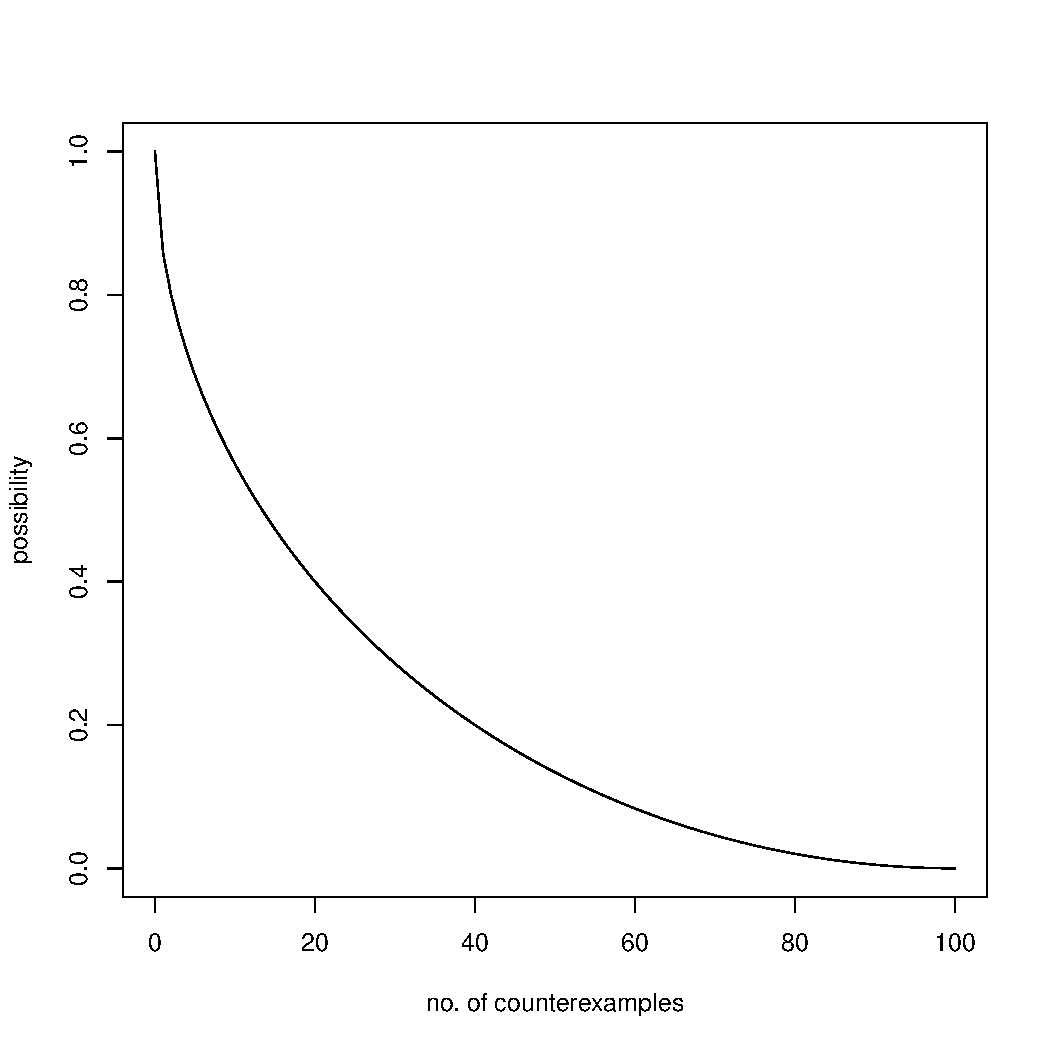
\includegraphics[width=2.25in]{../possibility} &
      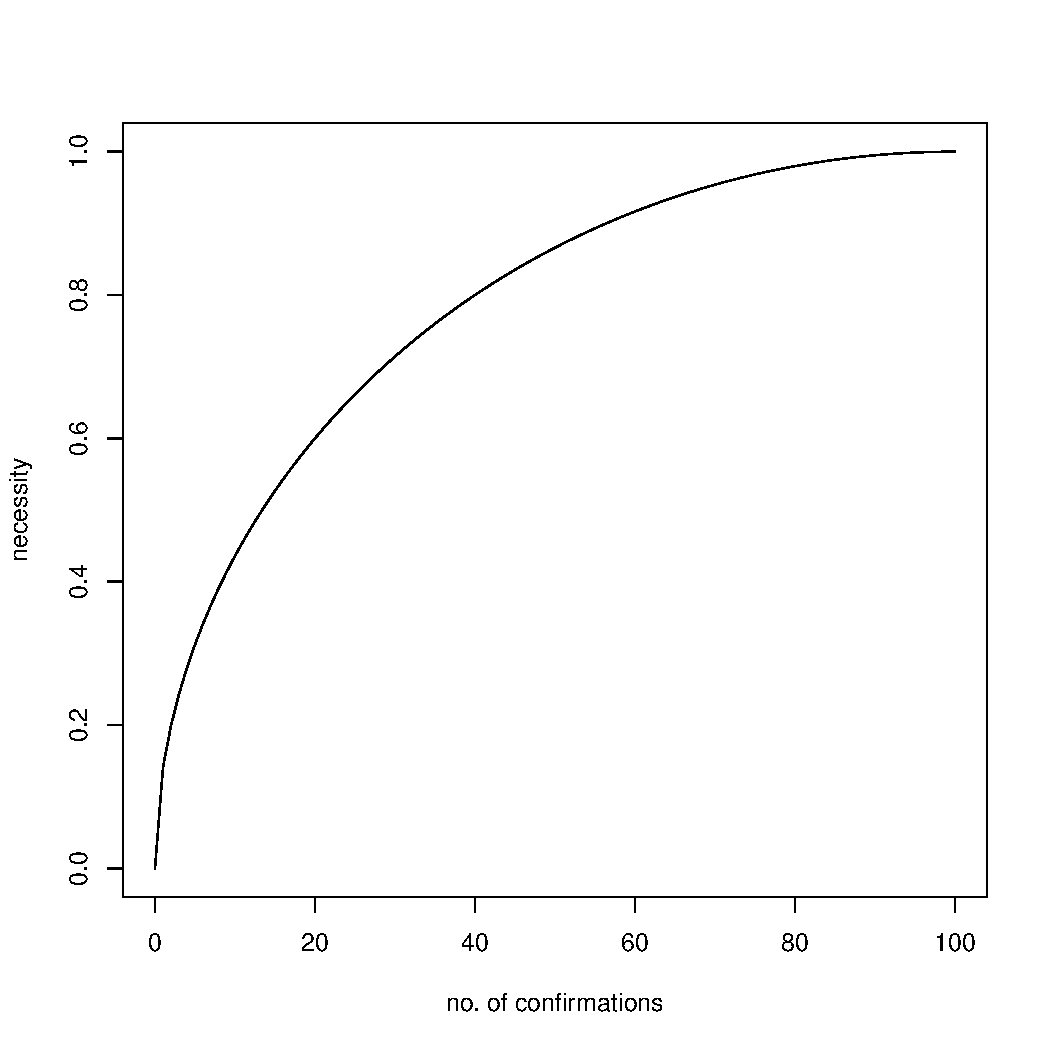
\includegraphics[width=2.25in]{../necessity} \\
      (a) & (b)
    \end{tabular}
  \end{center}
  \caption{A plot of $\Pi(\phi)$  as a function of
    $u_\phi^-$ (a) and of $N(\phi)$ as a function of
    $u_\phi^+$ (b) when $u_\phi = 100$.\label{fig:poss-nec-plots}}
\end{figure}

\subsection{Axiom Scoring}

We combine the possibility and necessity of an axiom to define
a single handy acceptance/rejection index (ARI) as follows:%
\footnote{The suggestion that this type of representation
may simplify the treatment of possibilistic uncertainty in some contexts
goes back to~\cite{GarciaMolinaRiosCardenosa1991}.}
\begin{equation}\label{eq:ARI}
  \mathrm{ARI}(\phi) = N(\phi) - N(\neg\phi) = N(\phi) + \Pi(\phi) - 1 \in [-1, 1].
\end{equation}
A negative $\mathrm{ARI}(\phi)$ suggests rejection of $\phi$ ($\Pi(\phi)<1$),
whilst a positive $\mathrm{ARI}(\phi)$ suggests its acceptance ($N(\phi)>0$),
with a strength proportional to its absolute value. A value close to zero
reflects ignorance about the status of $\phi$.
Figure~\ref{fig:ARI-plots} shows $\mathrm{ARI}(\phi)$  as a function of
$u_\phi^-$ and $u_\phi^+$ in the two cases of a $\phi$ whose development
is a conjunction or a disjunction, respectively, of basic statements.

\begin{figure}[t]
  \begin{center}
    \begin{tabular}{cc}
      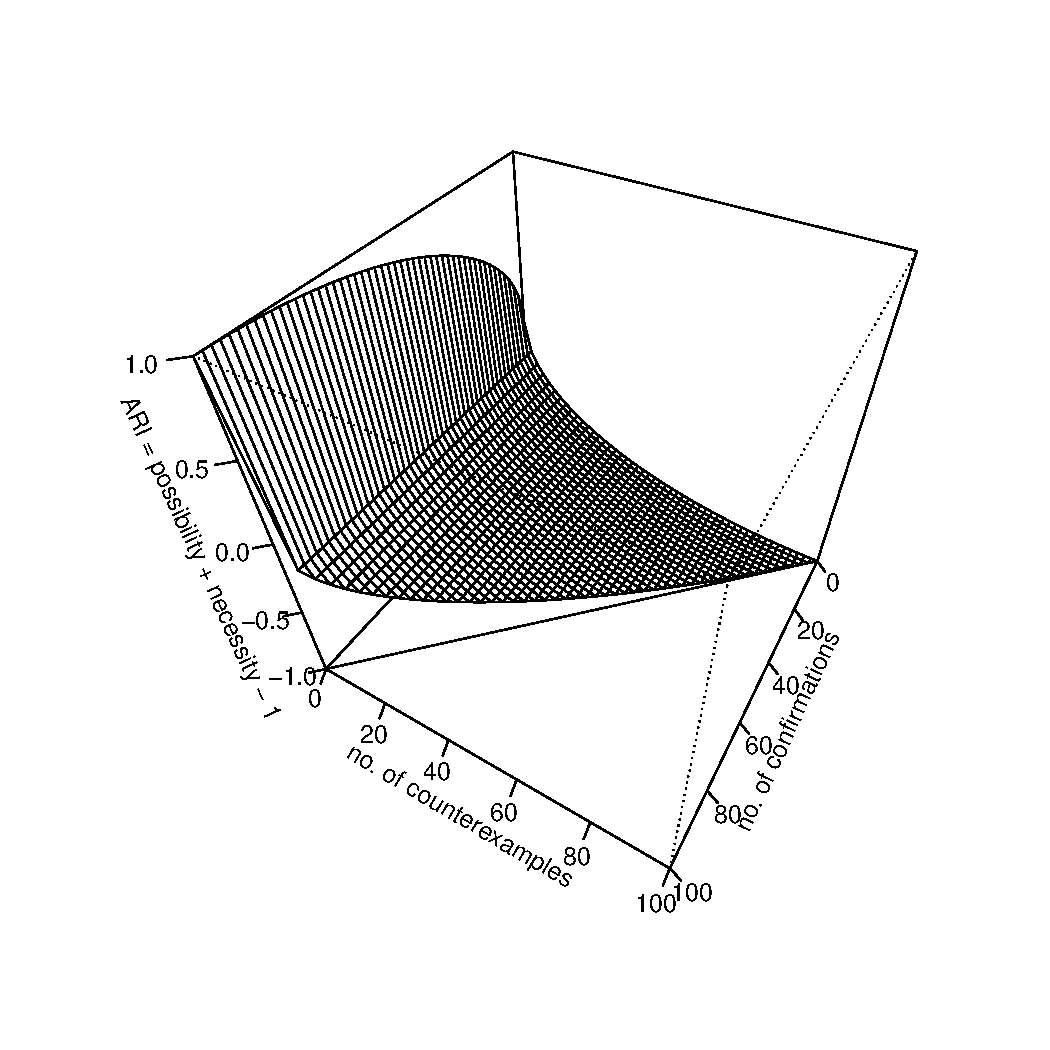
\includegraphics[width=2.25in]{../ARI-c} &
      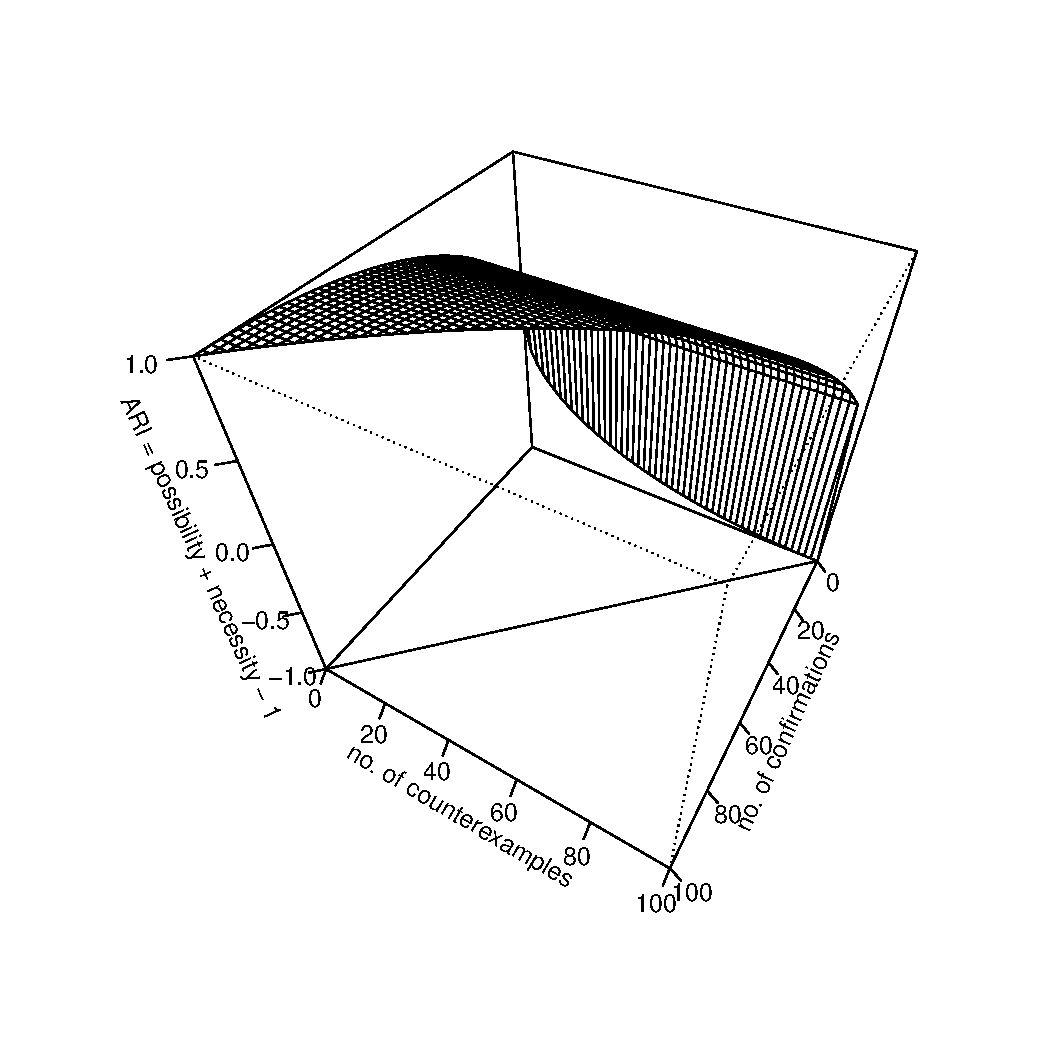
\includegraphics[width=2.25in]{../ARI-d} \\
      (a) & (b)
    \end{tabular}
  \end{center}
  \caption{Two plots of $\mathrm{ARI}(\phi)$ as a function of
    $u_\phi^-$ and $u_\phi^+$: (a) when $\phi$ has a conjunctive development and
     (b) when $\phi$ has a disjunctive development.\label{fig:ARI-plots}}
\end{figure}

Although this ARI is useful for the purpose of analyzing the results of our
experiments and to visualize the distribution of the tested axiom with respect
to a single axis, one should always bear in mind that an axiom is scored by
the proposed heuristics in terms of two bipolar figures of merit,
whose meanings, though related, are very different:
\begin{itemize}
\item $\Pi(\phi)$ expresses the degree to which $\phi$ may be considered ``normal'',
  in the sense of ``not exceptional, not surprising'', or not contradicted by
  actual observations;
\item $N(\phi)$, on the other hand, expresses the degree to which $\phi$ is
  certain, granted by positive evidence and corroborated by actual observations.
\end{itemize}


\section{Application to \texttt{SubClassOf} Axiom Testing}
\label{OWL2SPARQL} 

To illustrate how the theory developed in the previous sections can be
applied in practice, we summarize here an application to \texttt{SubClassOf}
axiom testing, developed in~\cite{TettamanziFaronZuckerGandon2014ekaw,%
TettamanziFaronZuckerGandon2015kcap}.
Scoring these axioms with their ARI requires to compute the development
of \texttt{Class} entities and \texttt{ObjectComplementOf} expressions. 
 
We define a mapping $Q(E, \mbox{\tt ?x})$ from OWL~2 class expressions to SPARQL graph patterns,
where $E$ is an OWL~2 class expression, and $\mbox{\tt ?x}$ is a variable,
such that the query
\texttt{SELECT DISTINCT ?x WHERE \{} $Q(E, \mbox{\tt ?x})$ \texttt{\}}
returns all the individuals which are instances of $E$. We denote this set by
$[Q(E, \mbox{\tt ?x})]$:
\begin{equation}
[Q(E, \mbox{\tt ?x})] = \{ v : (?x, v) \in ResultSet(\mbox{\tt SELECT DISTINCT ?x WHERE} \{ Q(E, \mbox{\tt ?x}) \} \}.
\end{equation} 

For a \texttt{Class} entity $A$, 
\begin{equation}
Q(A, \mbox{\tt ?x}) = \{\mbox{\tt ?x a }A \},
\end{equation}
where $A$ is a valid IRI.

For an \texttt{ObjectComplementOf} expression, things are slightly more complicated, since RDF does not support
negation. The model-theoretic semantics of OWL class expressions of the form \texttt{ObjectComplementOf(}$C$\texttt{)}
($\neg C$ in DL syntax), where $C$ denotes a class, is $\Delta^\mathcal{I} \setminus C^\mathcal{I}$.
However, to learn axioms from an RDF dataset, the open-world hypothesis must be made: the absence of
supporting evidence does not necessarily contradict an axiom, moreover an axiom might
hold even in the face of a few counterexamples.
%For example, for 143 out of 541 \texttt{SubClassOf} axioms in the DBpedia
%ontology, no resource in the DBpedia dataset provides any evidence;
%for 28, at least one counterexample is found in DBpedia 3.9.
%Axiom \texttt{SubClassOf(dbo:Person dbo:Agent)} even has 76 counterexamples!
%\todo{voir si on veut virer le paragraphe ci-dessus}
Therefore, as proposed in~\cite{TettamanziFaronZuckerGandon2014ekaw}, we define
$Q(\neg C, \mbox{\tt ?x})$ as follows, to approximate an open-world semantics:
\begin{equation}\label{eq:approx-open-world-negation}
  Q(\neg C, \mbox{\tt ?x}) =
  \begin{minipage}[t]{2in}
    \begin{tabbing}
      \quad\=\quad\=\quad\=\kill
      \{\>\texttt{?x a ?dc .}\\
        \>\texttt{FILTER NOT EXISTS} \{ \texttt{?z a ?dc . } $Q(C, \mbox{\tt ?z})$ \texttt{\} \}},
    \end{tabbing}
  \end{minipage}
\end{equation}
where \texttt{?z} is a variable that does not occur anywhere else in the query.

For a \texttt{Class} entity $A$, this becomes
\begin{equation}
Q(\neg A, \mbox{\tt ?x}) = \{\>\texttt{?x a ?dc . } \mbox{\tt FILTER NOT EXISTS } \{ \mbox{\tt ?z a ?dc . ?z a }A \} \}.
\end{equation}

A computational definition of $u_{C \sqsubseteq D}$ is the following SPARQL query:
\begin{equation}
  \begin{minipage}[c]{5in}
    \begin{tabbing}
      \quad\=\quad\=\quad\=\kill
      \texttt{SELECT (count(DISTINCT ?x) AS ?u)}\\
      \texttt{WHERE} \{$Q(C, \mbox{\tt ?x})$\}.
    \end{tabbing}
  \end{minipage}
\end{equation}


In order to compute the score of \texttt{SubClassOf} axioms, $ARI(C \sqsubseteq D)$, we must provide a computational definition of $u^+_{C \sqsubseteq D}$ and $u^-_{C \sqsubseteq D}$, respectively:
\begin{equation}
  \begin{minipage}[c]{5in}
    \begin{tabbing}
      \quad\=\quad\=\quad\=\kill
      \texttt{SELECT (count(DISTINCT ?x) AS ?nConfirm)}\\
      \texttt{WHERE} \{ $Q(C, \mbox{\tt ?x})$ $Q(D, \mbox{\tt ?x})$ \}
    \end{tabbing}
  \end{minipage}
\end{equation}
and
\begin{equation}
  \begin{minipage}[c]{5in}
    \begin{tabbing}
      \quad\=\quad\=\quad\=\kill
      \texttt{SELECT (count(DISTINCT ?x) AS ?nCounter)}\\
      \texttt{WHERE} \{ $Q(C, \mbox{\tt ?x})$ $Q(\neg D, \mbox{\tt ?x})$ \}.
    \end{tabbing}
  \end{minipage}
\end{equation}

The results of our first experiments described below
showed that an axiom which takes too long to test will likely end up having a very negative score.
We defined two heuristics based on this idea.
\begin{itemize}
%Fabien: intéressante subtilité:
%le graphique colorié (l'analyse comparative avec possibility) montre bien le premier point mais pas le deuxième.
%cath: on l'a viré ce graphique, il faut qu'on le montre autrement
%pour cela il faudrait associer une couleur allant de vert à jaune mais cette fois avec vert pour les axiomes ont été trouvé au début de la session de calcul et jaune pour celles qui ont été trouvées à la fin afin de voir la progression dans l'espace de recherche.
%cath: en fait il semble que ce ne sois pas très pertinent comme heuristique au vu du dernier graphique produit alors qu'on avait vu que si il y a un certain temps... je ne comprends plus rien mais il est tard.
\item We time-cap the SPARQL queries to compute the ARI of a candidate axiom and decide whether to accept or reject it, since above a computation time threshold, the axiom being tested is likely to get a negative ARI and be rejected.
\item We construct candidate axioms of the form $C \sqsubseteq D$, by considering
the subclasses $C$ in increasing order of the number of classes $D$ sharing at least
one instance with $C$.
This enables us to maximize the number of tested and accepted axioms in a given time period,
since it appears that the time it takes to test $C \sqsubseteq D$ increases with that number
and the lower the time, the higher the ARI.
\end{itemize}

We evaluated the proposed scoring heuristics by performing tests of \texttt{SubClassOf}
axioms using DBpedia 3.9 in English as the reference RDF fact repository.
In particular, on April 27, 2014, we downloaded the DBpedia dumps of English version 3.9,
generated in late March/early April 2013, along with the DBpedia ontology, version 3.9.
This local dump of DBpedia, consisting of 812,546,748 RDF triples,
with materialized inferences,
has been bulk-loaded into Jena TDB and a prototype
for performing axiom tests using the proposed method has been coded in Java,
using Jena ARQ and TDB to access the RDF repository.

We systematically generated and tested \texttt{SubClassOf} axioms
involving atomic classes only according to the following protocol:
for each of the 442 classes $C$ referred to in the RDF repository,
we construct all axioms of the form $C \sqsubseteq D$ such that $C$ and $D$
share at least one instance. Classes $D$ are obtained with the following query: 
\[
  \mbox{\tt SELECT DISTINCT ?D WHERE} \{ Q(C, \mbox{\tt ?x}) \mbox{\tt\ . ?x a ?D} \}.
\]

We experimentally fixed to 20 min the threshold to time-cap the SPARQL queries to compute $u^+_{C \sqsubseteq D}$ and $u^-_{C \sqsubseteq D}$
in order to decide whether to accept or reject a candidate axiom $C \sqsubseteq D$.

An in-depth quantitative and qualitative analysis of our experimental results is reported in~\cite{TettamanziFaronZuckerGandon2014ekaw} and \cite{TettamanziFaronZuckerGandon2015kcap}. Here we summarize the main findings.

We tested 5050 axioms using the time-capping heuristics.
Of these, 632 have been also tested without time capping, which is much more
expensive in terms of computing time by a factor of 142;
the outcome of the test was different on just 25 of them, which
represents an error rate of 3.96\%, a very reasonable price to pay,
in terms of accuracy degradation, in exchange for faster testing.
It should be observed that, by construction, these errors are all in the same
direction, i.e., some axioms which should be accepted are in fact rejected:
our heuristics are conservative, since they do not generate false positives.

Validating the results of our scoring heuristics in absolute term would require
having a knowledge engineer tag as true or false every axiom tested and compare
her judgment with the test score. Some insights gained from trying to do so
are given in~\cite{TettamanziFaronZuckerGandon2015kcap},
but besides being an extremely tedious and error-prone task,
manual evaluation is not completely reliable.

In order to obtain a more objective evaluation, 
we took all \texttt{SubClassOf}
axioms in the DBpedia ontology and added to them all \texttt{SubClassOf} axioms
that can be inferred from them, thus obtaining a ``gold standard'' of axioms
that \emph{should} be all considered as valid. 
This, at least, looks like a reasonable assumption, despite the fact that
in~\cite{TettamanziFaronZuckerGandon2014ekaw}
a number of potential issues were pointed out with the subsumption axioms
of the DBpedia ontology.
Of the 5050 tested axioms, 1915 occur in the gold standard; of these, 327 get an
ARI below 1/3, which would yield an error rate of about 17\%.
In fact, in most cases, the ARI of these axioms is around zero, which means that
our heuristic gives a suspended judgment.
Only 34 axioms have an ARI below $-1/3$. If we took these latter as the real errors,
the error rate would fall to just 1.78\%.

% Inserted in response to remarks by Reviewer #2
Finally, a comparison of the proposed scoring heuristic with a probabilistic
score, summarized in Figure~\ref{fig:ARI-BLS-dtc}, highlights some remarkable
differences in behavior. In the figure, each axiom is plotted according to its
ARI (X-axis) and its probabilistic score computed as in~\cite{BuehmannLehmann2012}
(Y-axis). First of all it is clear that both scores tend to agree in the extremes,
with some notable exceptions, but behave quite differently in all other cases.
With very few exceptions, all the axioms in the bottom right rectangle are
false negatives for the probabilistic score; most axioms in the upper left rectangle
are false positives. In addition, the color of the axioms is a function
of the time it took to compute their ARI (according to a terrain color scale)

\begin{figure}[t]
\begin{center}
  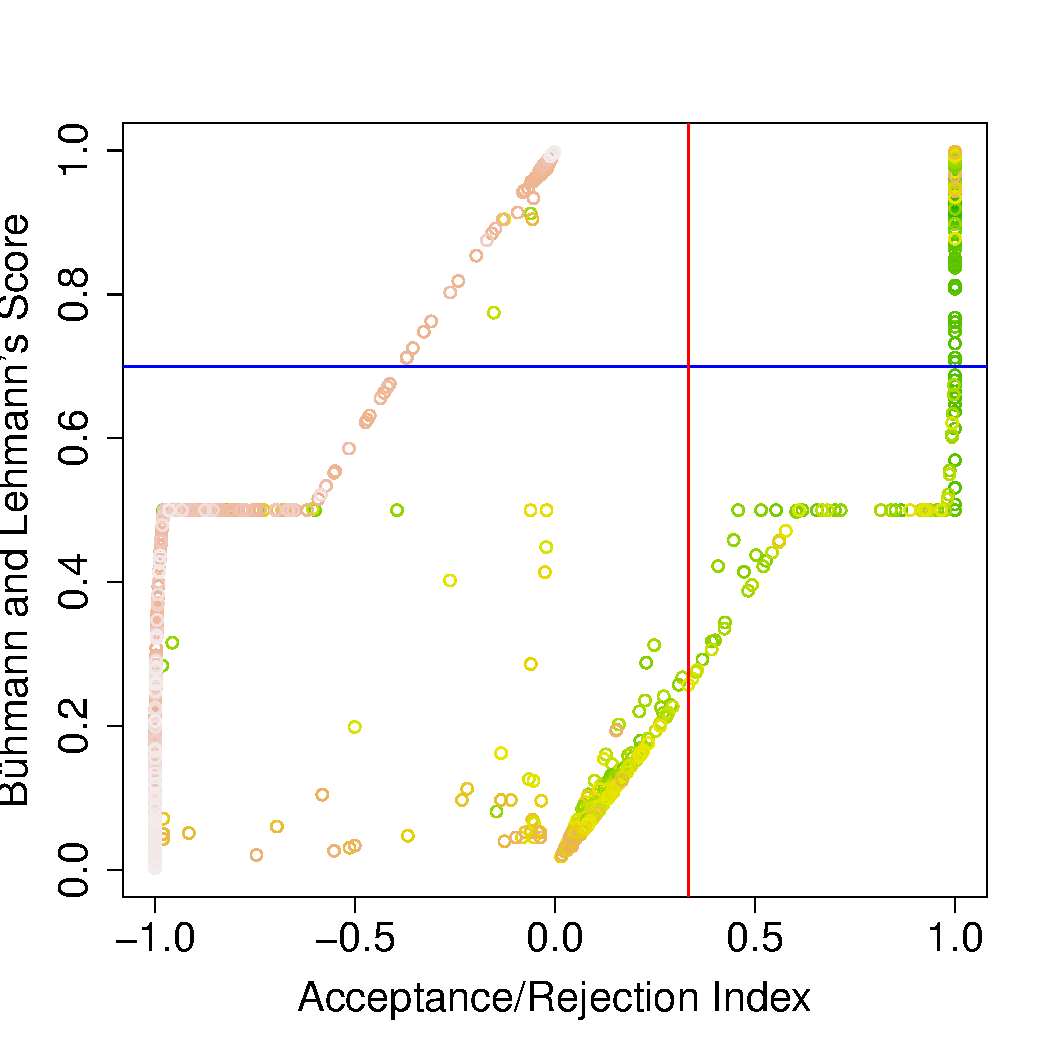
\includegraphics[height=3in]{ARI-BLS-dtc}
\end{center}
\caption{A comparison of the acceptance/rejection index and the probability-based
  score used in~\cite{BuehmannLehmann2012} on axioms tested with time capping.
  The vertical red line shows the acceptance threshold $\mathrm{ARI}(\phi)>1/3$;
  the horizontal blue line the acceptance threshold of 0.7 for the probabilistic score.}
\label{fig:ARI-BLS-dtc}
\end{figure}

On the 380 axioms tested in~\cite{TettamanziFaronZuckerGandon2014ekaw}
without time capping,
the probabilistic score with the 0.7 threshold suggested by~\cite{BuehmannLehmann2012}
gave 13 false negatives (7 more than the ARI) and 4 false positives
(one more than the ARI).
It was observed that most false axiom candidates got an ARI close to $-1$,
whilst their probabilistic scores are almost evenly distributed between 0 and 0.5,
which led us to argue that, besides being more accurate,
ARI gives clearer indications than the probabilistic score.

The increased accuracy and clarity of the possibilistic score come to a somehow
expensive price: we do not have precise figures, but the computational overhead
introduced by considering the possibilistic approach instead of a simpler
probabilistic score is orders of magnitude higher. The source of such dramatic
increase in cost is the execution of the SPARQL query
in Equation~\ref{eq:approx-open-world-negation} to approximate the semantics
of open-world negation.
While it is true that such a query is an integral part of our proposal,
one could argue that any probabilistic model wishing to take the open-world
assumption into account would have to incur similar costs; furthermore,
it is possible that SPARQL query execution engines can be optimized to make
the execution of queries of that type significantly faster.


\section{Conclusion}\label{conclusion}


We have developed the theory of a possibilistic framework for OWL~2 axiom testing
as an alternative to statistics-based heuristics.

The practical application of such a framework has been demonstrated by studying
the case of \texttt{SubClassOf} axiom testing against the DBpedia database.

A qualitative analysis of the results confirms the interest of using possibilistic
axiom scoring heuristics like the one we propose not only to learn axioms from the LOD,
but also to drive the validation and debugging of ontologies and RDF datasets.

Future research directions include the systematic computational definition
of the content of each kind of OWL~2 axioms, taking into account the principle
of selective confirmation. Based on it, we will continue our experiments
by testing the possibilistic framework on domain specific datasets
and extending it to test other types of OWL axioms, beginning with
\texttt{SubObjectPropertyOf} and \texttt{SubDataPropertyOf} axioms
and \texttt{SubClassOf} axioms involving\break\texttt{ObjectSomeValuesFrom}
class expressions.

%\section*{Acknowledgments}
%The authors would like to thank\dots

% \bibliography{../RDFMining}
\begin{thebibliography}{10}
\expandafter\ifx\csname url\endcsname\relax
  \def\url#1{\texttt{#1}}\fi
\expandafter\ifx\csname urlprefix\endcsname\relax\def\urlprefix{URL }\fi
\expandafter\ifx\csname href\endcsname\relax
  \def\href#1#2{#2} \def\path#1{#1}\fi

\bibitem{MaedcheStaab2001}
A.~Maedche, S.~Staab, Ontology learning for the semantic web, {IEEE}
  Intelligent Systems 16~(2) (2001) 72--79.
\newblock \href {http://dx.doi.org/10.1109/5254.920602}
  {\path{doi:10.1109/5254.920602}}.

\bibitem{LehmannVoelker2014}
J.~Lehmann, J.~V\"olker (Eds.), Perspectives on Ontology Learning, Vol.~18 of
  Studies on the Semantic Web, IOS Press, Amsterdam, 2014.
\newblock \href {http://dx.doi.org/10.3233/978-1-61499-379-7-i}
  {\path{doi:10.3233/978-1-61499-379-7-i}}.

\bibitem{FanizziDAmatoEsposito2008}
N.~Fanizzi, C.~d'Amato, F.~Esposito, {DL-FOIL} concept learning in description
  logics, in: F.~Zelezn{\'y}, N.~Lavrac (Eds.), Inductive Logic Programming,
  18th International Conference, ILP 2008, Prague, Czech Republic, September
  10-12, 2008, Proceedings, Vol. 5194 of Lecture Notes in Computer Science,
  Springer, 2008, pp. 107--121.
\newblock \href {http://dx.doi.org/10.1007/978-3-540-85928-4_12}
  {\path{doi:10.1007/978-3-540-85928-4_12}}.

\bibitem{FleischhackerVoelkerStuckenschmidt2012}
D.~Fleischhacker, J.~V{\"o}lker, H.~Stuckenschmidt, Mining {RDF} data for
  property axioms, in: R.~Meersman, H.~Panetto, T.~S. Dillon, S.~Rinderle-Ma,
  P.~Dadam, X.~Zhou, S.~Pearson, A.~Ferscha, S.~Bergamaschi, I.~F. Cruz (Eds.),
  On the Move to Meaningful Internet Systems: OTM 2012, Confederated
  International Conferences: CoopIS, DOA-SVI, and ODBASE 2012, Rome, Italy,
  September 10-14, 2012. Proceedings, Part II, Vol. 7566 of Lecture Notes in
  Computer Science, Springer, Berlin, 2012, pp. 718--735.
\newblock \href {http://dx.doi.org/10.1007/978-3-642-33615-7_18}
  {\path{doi:10.1007/978-3-642-33615-7_18}}.

\bibitem{HellmannLehmannAuer2009}
S.~Hellmann, J.~Lehmann, S.~Auer, Learning of {OWL} class descriptions on very
  large knowledge bases, Int. J. Semantic Web Inf. Syst. 5~(2) (2009) 25--48.
\newblock \href {http://dx.doi.org/10.4018/jswis.2009040102}
  {\path{doi:10.4018/jswis.2009040102}}.

\bibitem{BuehmannLehmann2012}
L.~B{\"u}hmann, J.~Lehmann, Universal {OWL} axiom enrichment for large
  knowledge bases, in: A.~ten Teije, J.~V{\"o}lker, S.~Handschuh,
  H.~Stuckenschmidt, M.~d'Aquin, A.~Nikolov, N.~Aussenac-Gilles, N.~Hernandez
  (Eds.), Knowledge Engineering and Knowledge Management - 18th International
  Conference, EKAW 2012, Galway City, Ireland, October 8-12, 2012. Proceedings,
  Vol. 7603 of Lecture Notes in Computer Science, Springer, 2012, pp. 57--71.
\newblock \href {http://dx.doi.org/10.1007/978-3-642-33876-2_8}
  {\path{doi:10.1007/978-3-642-33876-2_8}}.

\bibitem{ILPat20}
S.~Muggleton, L.~{De Raedt}, D.~Poole, I.~Bratko, P.~Flach, K.~Inoue,
  A.~Srinivasan, {ILP} turns 20: Biography and future challenges, Machine
  Learning 86 (2012) 3--23.
\newblock \href {http://dx.doi.org/10.1007/s10994-011-5259-2}
  {\path{doi:10.1007/s10994-011-5259-2}}.

\bibitem{GangemiCatenacciCiaramitaLehmann2005}
A.~Gangemi, C.~Catenacci, M.~Ciaramita, J.~Lehmann, A theoretical framework for
  ontology evaluation and validation, in: P.~Bouquet, G.~Tummarello (Eds.),
  SWAP 2005 - Semantic Web Applications and Perspectives, Proceedings of the
  2nd Italian Semantic Web Workshop, University of Trento, Trento, Italy, 14-16
  December 2005, Vol. 166 of CEUR Workshop Proceedings, CEUR-WS.org, 2005, p.
  Article No.: 2.

\bibitem{GangemiCatenacciCiaramitaLehmann2006}
A.~Gangemi, C.~Catenacci, M.~Ciaramita, J.~Lehmann, Modelling ontology
  evaluation and validation, in: Y.~Sure, J.~Domingue (Eds.), The Semantic Web:
  Research and Applications, 3rd European Semantic Web Conference, ESWC 2006,
  Budva, Montenegro, June 11-14, 2006, Proceedings, Vol. 4011 of Lecture Notes
  in Computer Science, Springer, 2006, pp. 140--154.
\newblock \href {http://dx.doi.org/10.1007/11762256_13}
  {\path{doi:10.1007/11762256_13}}.

\bibitem{TartirBudakArpinarSheth2007}
S.~Tartir, I.~{Budak Arpinar}, A.~P. Sheth, Ontological evaluation and
  validation, in: R.~Poli, M.~Healy, A.~Kameas (Eds.), Theory and Applications
  of Ontologies: Computer Applications, Springer, 2010, pp. 115--130.
\newblock \href {http://dx.doi.org/10.1007/978-90-481-8847-5_5}
  {\path{doi:10.1007/978-90-481-8847-5_5}}.

\bibitem{PovedaSuarezGomez2012}
M.~Poveda-Villal{\'o}n, M.~del Carmen Su{\'a}rez-Figueroa,
  A.~G{\'o}mez-P{\'e}rez, Validating ontologies with {OOPS}!, in: A.~ten Teije,
  J.~V{\"o}lker, S.~Handschuh, H.~Stuckenschmidt, M.~d'Aquin, A.~Nikolov,
  N.~Aussenac-Gilles, N.~Hernandez (Eds.), Knowledge Engineering and Knowledge
  Management - 18th International Conference, EKAW 2012, Galway City, Ireland,
  October 8-12, 2012. Proceedings, Vol. 7603 of Lecture Notes in Computer
  Science, Springer, 2012, pp. 267--281.
\newblock \href {http://dx.doi.org/10.1007/978-3-642-33876-2_24}
  {\path{doi:10.1007/978-3-642-33876-2_24}}.

\bibitem{FernandezGomezJuristo1997}
M.~Fern\'andez, A.~G\'omez-P\'erez, N.~Juristo, {METHONTOLOGY}: From
  ontological art towards ontological engineering, Tech. Rep. SS-97-06, AAAI
  (1997).

\bibitem{SirinTao2009}
E.~Sirin, J.~Tao, Towards integrity constraints in {OWL}, in: R.~Hoekstra,
  P.~F. Patel-Schneider (Eds.), Proceedings of the 5th International Workshop
  on OWL: Experiences and Directions (OWLED 2009), Chantilly, VA, United
  States, October 23--24, 2009, Vol. 529 of CEUR Workshop Proceedings,
  CEUR-WS.org, 2009, p. Article No.: 9.

\bibitem{KontokostasWestphalAuerHellmannLehmannCornelissen2014}
D.~Kontokostas, P.~Westphal, S.~Auer, S.~Hellmann, J.~Lehmann, R.~Cornelissen,
  A.~Zaveri, Test-driven evaluation of linked data quality, in: Proceedings of
  the 23rd International Conference on World Wide Web, International World Wide
  Web Conferences Steering Committee, Geneva, Switzerland, 2014, pp. 747--758.
\newblock \href {http://dx.doi.org/10.1145/2566486.2568002}
  {\path{doi:10.1145/2566486.2568002}}.

\bibitem{TettamanziFaronZuckerGandon2014ekaw}
A.~G.~B. Tettamanzi, C.~Faron-Zucker, F.~L. Gandon, Testing {OWL} axioms
  against {RDF} facts: A possibilistic approach, in: K.~Janowicz, S.~Schlobach,
  P.~Lambrix, E.~Hyv\"{o}nen (Eds.), Knowledge Engineering and Knowledge
  Management - 19th International Conference, {EKAW} 2014, Link{\"{o}}ping,
  Sweden, November 24-28, 2014. Proceedings, Vol. 8876 of Lecture Notes in
  Artificial Intelligence, Springer, 2014, pp. 519--530.
\newblock \href {http://dx.doi.org/10.1007/978-3-319-13704-9_39}
  {\path{doi:10.1007/978-3-319-13704-9_39}}.

\bibitem{TettamanziFaronZuckerGandon2015kcap}
A.~G.~B. Tettamanzi, C.~Faron-Zucker, F.~Gandon, Dynamically time-capped
  possibilistic testing of subclassof axioms against rdf data to enrich
  schemas, in: K.~Barker, J.~M. G\'omez-P\'erez (Eds.), K-CAP 2015. Proceedings
  of the 8th International Conference on Knowledge Capture, Palisades, NY, USA,
  October 07--10, 2015, ACM, New York, 2015, p. Article No.: 7.
\newblock \href {http://dx.doi.org/10.1145/2815833.2815835}
  {\path{doi:10.1145/2815833.2815835}}.

\bibitem{QiPanJi2011}
G.~Qi, Q.~Ji, J.~Z. Pan, J.~Du, Extending description logics with uncertainty
  reasoning in possibilistic logic, International Journal of Intelligent
  Systems 26 (2011) 353--381.
\newblock \href {http://dx.doi.org/10.1002/int.20470}
  {\path{doi:10.1002/int.20470}}.

\bibitem{QiJiPanDu2010}
G.~Qi, Q.~Ji, J.~Z. Pan, J.~Du, {PossDL} -- {A} possibilistic {DL} reasoner for
  uncertainty reasoning and inconsistency handling, in: L.~Aroyo, G.~Antoniou,
  E.~Hyv{\"{o}}nen, A.~ten Teije, H.~Stuckenschmidt, L.~Cabral, T.~Tudorache
  (Eds.), The Semantic Web: Research and Applications, 7th Extended Semantic
  Web Conference, {ESWC} 2010, Heraklion, Crete, Greece, May 30 - June 3, 2010,
  Proceedings, Part {II}, Vol. 6089 of Lecture Notes in Computer Science,
  Springer, 2010, pp. 416--420.
\newblock \href {http://dx.doi.org/10.1007/978-3-642-13489-0_35}
  {\path{doi:10.1007/978-3-642-13489-0_35}}.

\bibitem{Crupi2016}
V.~Crupi,
  \href{https://plato.stanford.edu/archives/win2016/entries/confirmation/}{Confirmation},
  in: E.~N. Zalta (Ed.), The Stanford Encyclopedia of Philosophy, winter 2016
  Edition, Metaphysics Research Lab, Stanford University, 2016.
\newline\urlprefix\url{https://plato.stanford.edu/archives/win2016/entries/confirmation/}

\bibitem{OWL2-direct-semantics}
B.~{Cuenca Grau}, B.~Motik, P.~{Patel-Schneider},
  \href{http://www.w3.org/TR/2012/REC-owl2-direct-semantics-20121211/}{{OWL} 2
  web ontology language direct semantics (second edition)}, {W3C}
  recommendation, W3C (December 2012).
\newline\urlprefix\url{http://www.w3.org/TR/2012/REC-owl2-direct-semantics-20121211/}

\bibitem{Hempel1943}
C.~G. Hempel, A purely syntactical definition of confirmation, The Journal of
  Symbolic Logic 8~(4) (December 1943).

\bibitem{DLHandbook2003}
F.~Baader, D.~Calvanese, D.~McGuinness, D.~Nardi, P.~Patel-Schneider (Eds.),
  The Description Logic Handbook: Theory, implementation and applications,
  Cambridge, 2003.

\bibitem{SchefflerGoodman1972}
I.~Scheffler, N.~Goodman, Selective confirmation and the ravens: A reply to
  {Foster}, The Journal of Philosophy 69~(3) (1972) 78--83.

\bibitem{Agrawal1993}
R.~Agrawal, T.~Imielinski, A.~N. Swami, Mining association rules between sets
  of items in large databases, in: Proc. of the Int. Conf. on Management of
  Data, ACM Press, 1993, pp. 207--216.
\newblock \href {http://dx.doi.org/10.1145/170035.170072}
  {\path{doi:10.1145/170035.170072}}.

\bibitem{AgrestiCoull1998}
A.~Agresti, B.~A. Coull, Approximate is better than ``exact'' for interval
  estimation of binomial proportions, The American Statistician 52~(2) (May 1998).
\newblock \href {http://dx.doi.org/10.1080/00031305.1998.10480550}
  {\path{doi:10.1080/00031305.1998.10480550}}.

\bibitem{Lakoff1987}
G.~Lakoff, Women, Fire, and Dangerous Things, University Of Chicago Press,
  Chicago, 1987.

\bibitem{Sowa2000}
J.~F. Sowa, Knowledge Representation: Logical, Philosophical, and Computational
  Foundations, Brooks/Cole, Pacific Grove, CA, 2000.

\bibitem{Zadeh1978}
L.~A. Zadeh, Fuzzy sets as a basis for a theory of possibility, Fuzzy Sets and
  Systems 1 (1978) 3--28.

\bibitem{dubois1991}
D.~Dubois, H.~Prade, Fuzzy sets and probability: Misunderstandings, bridges and
  gaps, Fuzzy Sets and Systems 40~(1) (1991) 143--202.
\newblock \href {http://dx.doi.org/10.1109/FUZZY.1993.327367}
  {\path{doi:10.1109/FUZZY.1993.327367}}.

\bibitem{Popper1935}
K.~Popper, Logik der Forschung, Verlag von Julius Springer, Vienna, 1935.

\bibitem{GarciaMolinaRiosCardenosa1991}
J.~{Garc\'{\i}a del Real}, R.~G. Molina, J.~{R\'{\i}os Carri\'on},
  J.~{Carde\~nosa Lera}, A simplified technique for using necessity-possibility
  measures, International Journal of Approximate Reasoning 5~(4) (1991)
  399--413.
\newblock \href {http://dx.doi.org/10.1016/0888-613X(91)90019-I}
  {\path{doi:10.1016/0888-613X(91)90019-I}}.

\end{thebibliography}
\end{document}

